% psylab-doc.tex

\documentclass[a4paper]{article}
\usepackage[latin1]{inputenc}
%\usepackage[german]{babel}
\usepackage{graphicx,color,hyperref}
\usepackage{longtable}
\usepackage{makeidx}
\usepackage{struktex}

\setlength{\textwidth}{16cm}
\setlength{\oddsidemargin}{0cm}
\setlength{\textheight}{24cm}
\addtolength{\topmargin}{-1.8cm}

\newcommand{\psylabversion}{2.9}

\usepackage{fancyhdr}
\pagestyle{fancy}

\lhead{Version \psylabversion}
\rhead{\thepage}
\cfoot{}
\chead{\psylab\ - Documentation}


%% -----------------------------------------------------------------
%% Copyright (C) 2004-2008         Martin Hansen, FH OOW  
%% Author :  Martin Hansen,  <psylab AT jade-hs.de>
%% Date   :  14 Jan 2004
%% Updated:  <11 Feb 2019 14:53, martin>
%% Updated:  <29 Mai 2017 09:27, martin>
%% Updated:  <20 Feb 2017 14:41, martin>
%% Updated:  < 7 Nov 2016 14:18, martin>
%% Updated:  < 1 Nov 2011 08:58, martin>
%% Updated:  < 8 Feb 2008 15:33, hansen>
%% Updated:  <14 Jun 2007 11:59, hansen>
%% Updated:  <17 Apr 2007 12:01, hansen>
%% Updated:  <29 Mar 2007 22:56, hansen>
%% Updated:  <27 Nov 2006 22:33, hansen>
%% Updated:  <16 Jan 2006 21:09, mh>
%% Updated:  <16 Jan 2006 21:08, mh>
%% Updated:  < 8 Apr 2005 11:34, hansen>

%% This file is part of PSYLAB, at collection of scripts for
%% designing and controlling interactive psychoacoustical listening
%% experiments.  
%% This file is free software; you can redistribute it and/or modify
%% it under the terms of the GNU General Public License as published
%% by the Free Software Foundation; either version 2 of the License, 
%% or (at your option) any later version.  See the GNU General
%% Public License for more details:  http://www.gnu.org/licenses/gpl
%% This file is distributed in the hope that it will be useful,
%% but WITHOUT ANY WARRANTY.
%% PSYLAB is written in MATLAB, based on many ideas and concepts 
%% of its predecessor SISG/SI, a system originally written 
%% by Dirk Pueschel, Rene Koch, and Ralf Fassel in 1989-1991.

% the name of the game. 
\newcommand{\psylab}{{\sc PsyLab}}
% formatting for matlab code
\newcommand{\code}[1]{\texttt{#1}}
\newcommand{\ie}{i.\,e.\ }
\newcommand{\eg}{e.\,g.\ }

\newcommand{\fixme}[1]{
\fbox{\color{red}
{FIXME: }#1}
}


\title{\psylab\ -- Documentation\\ Version \psylabversion}
\author{Martin Hansen \\ 
Institut f�r H�rtechnik + Audiologie\\
Jade Hochschule\\
Oldenburg, Germany}
%\date{8. Januar 2006}

\makeindex

\begin{document}

\maketitle
% \begin{center}
% \section*{PSYLAB -- Documentation}
% Version: \today
% \end{center}

%\clearpage 
%\vfill
\vspace*{-6ex}
\tableofcontents
%\vfill
\clearpage


%% ============================================================
\section{Introduction}
\label{sec:introduction}

%% --------------------------------------------------
\subsection{What is \psylab?}
\label{sec:what-is-psylab}

'\psylab' is a collection of scripts, written in Matlab, for 
designing and controlling interactive psychoacoustical listening
experiments in a uniform and quick manner.

Currently, $n$-AFC detection and discrimination experiments
($n=2,3,4$) and 2-AFC matching experiments are readily supported.  The
stimulus variable can either be controlled adaptively according to
$x$-up-$y$-down algorithms ($x,y \in \{1,2,3\})$) and weighted-up-down
algorithms.  Alternatively, the method of constant stimuli may be used
for detection and discrimination experiments.


%% --------------------------------------------------
\subsection{History of  \psylab}
\label{sec:history-psylab}


\psylab\ is based on many ideas of the programs 'SI/SISG' which were
written at ``Drittes Physikalisches Institut'', Universit�t G�ttingen,
during the years 1989 to 1991, and which were distributed under the GNU
General Public License (GNU~GPL).
%
SI~(``Signalverarbeitung interaktiv'') was programmed in Fortran by
Dirk P�schel and Ren� Koch and further colleagues for the
purpose of digital signal processing and analysis.  SISG, built on
SI, was written by Ralf Fassel and was used for development, control
and analysis of psychoacoustical experiments.  The philosophy and
organisation of \psylab\ was inspired by the paradigms of ``SISG'' in
many ways. 

\psylab\ has been written by Martin Hansen.  It is regularly used for
education and research at Institut f�r H�rtechnik und Audiologie
(IHA), Jade Hochschule in Oldenburg, Germany.
% where it has been used intensively by many students.

One aim of \psylab\ has been to provide the students in the
psychoacoustic courses with a uniform and simple starting point for
designing one's own listening experiments.  So far, roughly 400
students at IHA have used \psylab\ in their psychoacoustics
assignments, for designing and carrying out individual listening
experiments.  Their experience and comments have continuously
contributed to new features and bug fixes of \psylab.


%% --------------------------------------------------
\subsection{License of \psylab}
\label{sec:licence-psylab}

\psylab\ is ``free software'' and is distributed in OpenSource format
under the terms of the GNU General Public License (GPL).  This means,
amongst others, that copies of the \psylab-software may be distributed
without asking for permission, given that the terms of the GNU GPL are
obeyed to.

For more details, see \texttt{http://www.gnu.org/licenses/} or look
at a verbose copy of the GNU GPL on page~\pageref{sec:gnu-gpl}.


%% --------------------------------------------------
\subsection{No warranty, no liability}
\label{sec:psylab-no-warranty}

\emph{  \psylab\ is distributed without any kind of warranty.
Have a look at the file ``\texttt{NO-WARRANTY}'' in the root directory of
\psylab\ before using it!}

The use of \psylab, for whatever purpose, is under the complete and
sole responsibility of the user.  \textcolor{red}{\textbf{Special attention is drawn to the
fact that \psylab\ does \emph{not} comprise an automatic mechanism to
prevent the delivery of too loud sound pressure levels.}}  It is the
explicit and sole responsibility of the user of \psylab\ to make sure that
the generated stimuli, in combination with any further equipment
(sound card, amplifier, headphone or loudspeaker, etc.), will yield the
desired sound level.  



%% --------------------------------------------------
\subsection{Quick start: example experiments}
\label{sec:quickstart-examples}


A hands-on explanation of the way how \psylab\ works can be found in
the subdirectory '\texttt{examples}' of the \psylab-distribution.  It
contains several example experiments, ready for giving them a try.

Each experiment is comprised of three scripts with similar names,
i.e., with the same first part of the name.  The name of the ``main
script'' of an experiment can be chosen freely, \eg
'\texttt{myscript.m}'.  The two accompanying scripts \emph{must} then
carry the names '\texttt{myscriptset.m}' and
'\texttt{myscriptuser.m}'.
% Note that the
% name of the main script serves as a prefix and that the keywords
% '\texttt{set}' and '\texttt{user}' follow directly after, i.e.\
% without any further character in between.  
The main script describes and controls the measurements while the
other two scripts are used for stimulus generation during the
experiment.  For a quick start, run one of the example experiments by
running the corresponding main script. 

The example in the file '\texttt{sam\_sincarrier\_detect.m}' is an
experiment which measures the detection threshold of the modulation
degree of sinusoidal amplitude modulation (``SAM'') as a function of
modulation frequency.  The measurements are performed for a number of
different carrier frequencies of the sinusoidal carrier.

The example in the file \texttt{jnd\_frequency.m} is an experiment
which measures frequency discrimination of pure sinusoids as a
function of the reference tone frequency and its sound level. 

The example in the file \texttt{match\_freq\_binaural.m} is a matching
experiment which measures the frequency for binaural pitch matching
between left and right ear for pure tones as a function of the
reference frequency. 

The example in the file \texttt{tone\_in\_broadbandnoise.m} is an
experiment with interleaved tracks for measuring the detection
threshold of the level of a sinusoid in broad band noise as a function
of the tone frequency.  

\section{Philosophy and structure of \psylab}
\label{sec:philosophy-psylab}


%% --------------------------------------------------
\subsection{Coding style in \psylab}
\label{sec:psylab-coding-style}

The coding style in \psylab\ may lead to some debate for some
people.  However, keep in mind that \psylab\ was not designed to serve
as an example for one or another coding style.   

For several reasons, amongst others easy accessibility for students
with limited prior experience in programming/coding, most of the
\psylab\ source files are written as \emph{scripts}/\emph{m-files}, i.e.\ not
as functions.  This means that all variables controlling \psylab's
behaviour reside in the global workspace of Matlab.  This makes it
especially important for the user to be informed about the specific
naming convention for files and variables.  This is explained in
section~\ref{sec:name-conventions}.


%% --------------------------------------------------
\subsection{Conventions in \psylab: reserved names for files and variables}
\label{sec:name-conventions}

An important convention respectively requirement of \psylab\ is that every
experiment must be made up of three (Matlab) scripts.  These are the
\index{scripts!main script}``main script'', the 
\index{scripts!set script}``set script'', and the 
\index{scripts!user script}``user script''.  These three files must be pure scripts, i.e.\ they may
\emph{not} be Matlab \emph{functions}!  As a consequence, the scripts
can access all variables of the global Matlab-workspace.  The scripts
can of course call further scripts or functions.  By defining the file
name of the main script, the names of the set script and the user
script are determined, too: Their names result from
concatenating '\texttt{set}' respectively '\texttt{user}' directly after the
name of the main script, \eg \texttt{testnameset.m} respectively 
\texttt{testnameuser.m} if the name of the main script is
\texttt{testname.m}.  Note that no single character is allowed between
the '\texttt{set}' or the '\texttt{user}' and the name of the main
script.

Another convention applies to the use of certain variables with
reserved names, \eg \code{M.VAR}, \code{M.PARAM}, \code{m\_ref},
\code{m\_test}.  See sections~\ref{sec:main-script},
\ref{sec:set-script}, \ref{sec:user-script},
\ref{sec:variables-controlling-psylab}. 



%% --------------------------------------------------
\subsection{Terminology and definitions}
\label{sec:terminology}

This section explains some terms and definitions used inside \psylab.   
In addition, the principal course of psychoacoustical experiments realised
with \psylab\ is explained.  Some of the terms are illustrated in
Fig.~\ref{fig:example_run}.  

\begin{description}

\item[interval, signal, stimulus] 
  
  During an experiment, the human test subject is presented with one
  or more stimuli.  The individual stimuli are also called
  \index{interval}intervals or signals.  In an $n$-AFC-experiment, $n$
  intervals are presented in succession.  Most often, these signal
  intervals will be separated by short pauses (of silence).  It is
  possible to visually mark the individual intervals.

\item [trial] 

  A \index{trial}trial is one presentation of the $n$ stimulus
  intervals that pertain to an $n$-AFC experiment.  After each trial
  the subject is required to answer respectively respond to a
  question, for example one of the kind ``which interval contained the
  test signal?''.

\item[(stimulus) variable] 

  The \index{stimulus variable}``variable'' inside \psylab\ takes the
  role of that stimulus dimension/magnitude which is varied from trial
  to trial (for example adaptively, or using a method of constant
  stimuli) in order to find the subject's threshold.  The ``variable''
  carries the reserved name \code{M.VAR} inside \psylab.

\item[(stimulus) step size] 

  The \index{step size} step size is the magnitude by which the
  stimulus variable gets changed from trial to trial during an
  adaptive experiment.  It is measured in the same units of the
  variable \code{M.VAR}.  The step size is typically larger in the
  beginning of the experiment and is then progressively reduced until
  some minimal step size has been reached.  The step size carries the
  reserved name \code{M.STEP} inside \psylab, and the 
  \index{step size!minimal}minimal step size carries the name
  \code{M.MINSTEP}.

  The step size doesn't have a meaning and isn't used in the ``method
  of constant stimuli''. 

\item[run] 

  A \index{run}run is the succession of all trials that are necessary
  to reach and determine one threshold of the varying stimulus
  variable.

\item[(stimulus) parameter] 

  The \index{stimulus parameter}parameter inside \psylab\ has the
  meaning of the arbitrary (but then fixed) stimulus
  dimension/magnitude which is usually kept constant during one run
  until threshold has been established.  In the next run the stimulus
  parameter would then usually be set to another value and the
  corresponding threshold would again be established, and so on.  The
  ``parameter'' carries the reserved name \code{M.PARAM}.

\item[ 2nd, 3rd, ... (stimulus) parameter]

  If an experiment requires \index{stimulus parameter!more than one}more 
  than only one stimulus parameter, \psylab\ offers the possibility to
  use (and organise) any number of independent parameters.  In that
  case, \texttt{M.PARAM} will just be a vector instead of a scalar,
  and \code{M.PARAM(1)} will be the 1st parameter value,
  \code{M.PARAM(2)} the 2nd, \code{M.PARAM(3)} the 3rd, etc.

\item[reference signal] 

  In a trial of a $n$-AFC experiment, $n$ intervals are presented in
  succession, and in random order.  There are $n-1$ intervals among
  them which contain the \index{signals!reference signal}reference
  signal, i.e.\ they do \emph{not} contain ``the signal'' or the
  ``cue'' that the subject is required to detect.  The reference
  signal must carry the reserved name \code{m\_ref} \emph{or}
  \code{m\_ref1}, \code{m\_ref2} etc.\ inside \psylab.

\item[test signal] 
  
  The \index{signals!test signal}test signal is the signal which
  \emph{does} contains that special ``cue'' that the subject is
  required to detect, contrary to the reference signal which does not.
  The test signal will be presented at random in one of the $n$
  intervals of a $n$-AFC trial. The test signal must carry the
  reserved name \code{m\_test} inside \psylab.

\item[familiarisation phase] 

  At the beginning of a new run with an adaptive control of the
  stimulus variable, the test signal will typically be presented
  clearly above threshold in order to orient the subject about the
  kind of the signal respectively the ``cue'' that is to be detected,
  and to familiarise the subject with the measurement procedure.  The
  step size will be larger at the beginning of this
  \index{familiarisation phase}familiarisation phase so that correct
  responses of the subject will carry the stimulus variable towards
  the region of threshold more or less rapidly.  At the same time the
  step size will be reduced progressively until it has reached the
  minimal step size which the user has to specify.  The trials up to
  this point are only used for familiarisation of the subject, and to
  approach a value of the stimulus variable in the vicinity of the
  threshold.  The trials of the familiarisation phase will however
  \emph{not} be included in the determination of the threshold.

  When using the ``method of constant stimuli'', there is no
  familiarisation phase.  


\item[measurement phase] 

  In an adaptive run, the \index{measurement phase}measurement phase
  starts at the end of the familiarisation phase.  The subject should
  have approached a point relatively close to the threshold and the
  stimulus variable changes now only with the minimal step size.  The
  measurement phase lasts until a certain number of reversals (see
  below) has been reached.  This maximum number of reversals serves as
  a stop criterion and needs to be specified by the user.  The
  threshold is then estimated based on all values that the variable
  had taken on during the measurement phase.

\item[reversal / turning point]

  In a transformed-up-down experiment \cite{levitt_1971}, the stimulus
  variable and its direction of change depend on the subject's
  responses.  The direction alternates back and forth between ``going down''
  and ``going up''.  
\\
  \underline{\textbf{NB:}  Until version 2.5}, \psylab\ counted only an upper
    point, i.e.\ the change from an up-phase to
    the next down-phase as 1 \index{reversal}``reversal''.
\\
  \underline{\textbf{NB:}  Since version 2.6}, \psylab\ counts both an
  upper (from-up-to-down) and a lower (from-down-to-up) point as 1
  \index{reversal}``reversal''. 
%\\
\begin{quote}
  In other words, as of version 2.6, the occurrence of a local maximum, and
  likewise of a local minimum, of the stimulus variable \code{M.VAR} as a
  function of the trial number is defined as a reversal.  This
  definition inside \psylab\ is in line with the definition of
  ``reversals'' respective ``turning points'' in the majority of the literature.
\end{quote}
% 
  The number of reversals serves as a \index{stop criterion}stop
  criterion for a adaptive run.  When the number of reversals within the
  measurement phase has reached the
  \index{reversal!maximum number of}maximum number of reversals, as
  specified by \code{M.MAXREVERSAL}, that run is terminated.

  If you re-use an older experiment, implemented with \psylab\ version
  up to 2.5 using the old definition of reversals, there will be a
  (limited) automatic check for meaningful values of the variable
  \code{M.MAXREVERSAL}. 



\end{description}

%%
\begin{figure}[htb]
\begin{center}
  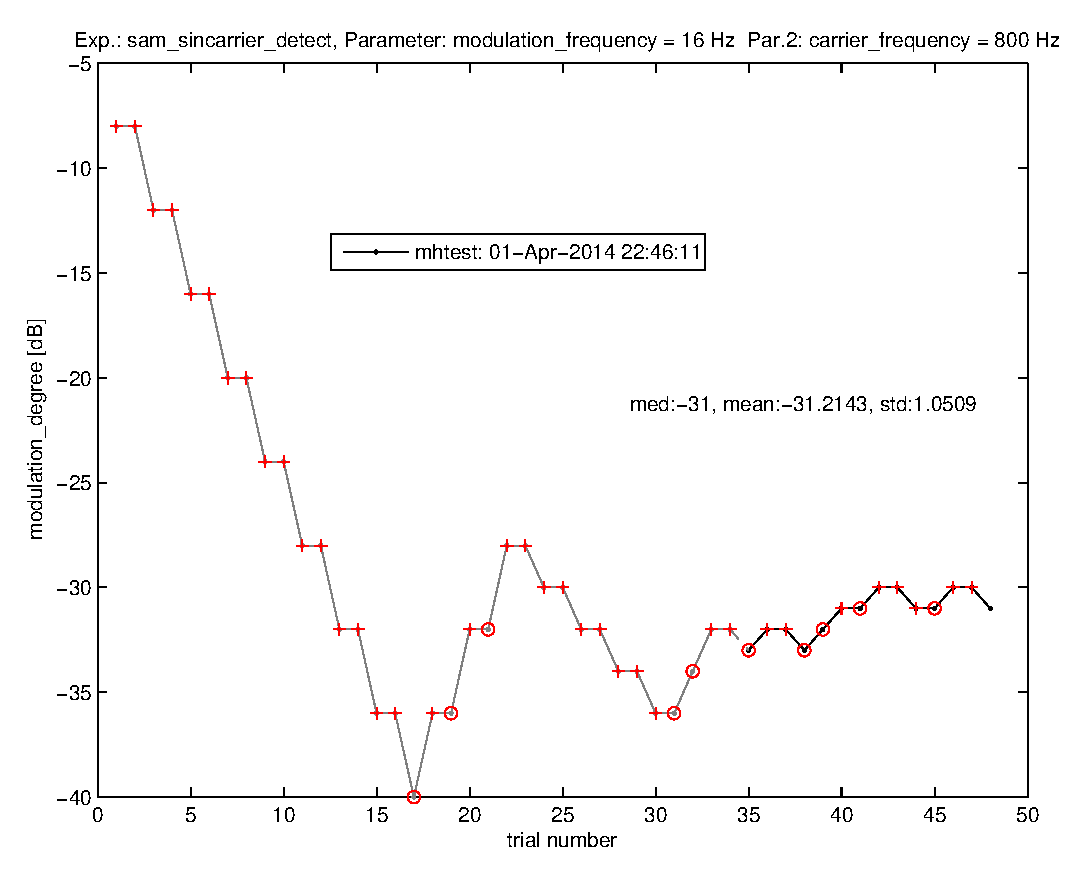
\includegraphics[width=0.75\textwidth]{example_run_reversals}
  \caption{Example of the course of one experimental run with \psylab.
    The plus-signs (+) mark a correct response of the subject, the
    circles ($\circ$) mark a wrong one. 
    % The arrows indicate the locations of a reversal.  
    The familiarisation phase (depicted in gray) lasted from trial 1 up to trial 34.
    During that phase reversals occurred at trial 17, 23, 31, and 34.  At
    each upper reversal, the step size was halved until the minimum
    step size of 1~dB had been reached. At that point, the measurement phase
    started (at trial 35, depicted in black) and it lasted for 6 reversals (at trials
    35, 37, 38, 43, 35, and 47) which had been
    set as the maximum number of reversals.  The last reversal of
    those 6 was reached in trial 47 and the run terminated there.  The
    very last data point, trial 48, \emph{would} have been presented
    next with a modulation degree as indicated, hadn't the run
    stopped.}
  \label{fig:example_run}
\end{center}
\end{figure}%
%%

Figure~\ref{fig:example_run} shows an example run of the experiment
\texttt{sam\_sincarrier\_detect.m} which can be found in the
subdirectory \texttt{examples} of the \psylab-distribution.  The data
show the value of the stimulus variable as a function of the trial
number.  The plot can be generated automatically with the
\psylab-script \texttt{mpsy\_display\_psydat.m}, see
section~\ref{sec:display-results}.  The run started with the
familiarisation phase with the settings \code{M.VAR = -8; M.STEP =
  4;}.  Both values are stated in dB re. 1.  The first reversal was
reached at trial~17, the step size remained at 4~dB.  At trial~23 the
second reversal was reached.  As this was an upper reversal, the step
size was halved to 2~dB.  At trial~31 the third reversal was
encountered and the step size remained at 2~dB.  At trial~34 the
fourth reversal was reached and the step size was halved to 1~dB.  As
this step size had been defined as the minimal step size, the
familiarisation phase ended here and the measurement phase started at
the next trial~35.  From there, the number of reversals starts again
counting from scratch.  The run terminated when a number of
\code{M.MAXREVERSAL} reversals had been reached.  In the example with
\code{M.MAXREVERSAL=6;} this point was reached after trial~47.  Note
that the plot shows a data point at trial 48 which was \emph{not}
presented to the subject.  The corresponding stimulus \emph{would}
have been presented to the subject, hadn't the run just been
terminated.  The threshold is calculated as the \emph{median} of all
values of \code{M.VAR} during the measurement phase, a value of -31~dB
in the example.  The standard deviation of the threshold is calculated
from the same data points and amounted to 1.05~dB in the example. The
mean of all data points in the measurement phase is also stated, but
only in the plot.




%% --------------------------------------------------
\subsection{Types of experiments in \psylab}
\label{sec:types-of-experiments-psylab}

\psylab\ offers to perform various kinds of experiments.  One class of
experiments are detection and discrimination experiments using a
$N$-AFC transformed-up-down method.  These experiments can be
performed as a sequence of single runs, one run at a time, or as a group
of interleaved runs.  These are described in
sections~\ref{sec:n-afc-experiments} resp.\
\ref{sec:interleaved-experiments}.

Slightly different are matching experiments, like for example employed
in pitch matching or loudness matching.  The difference relative to
$N$-AFC detection experiments is that the answer of the subject can
not be judged to be correct or wrong.  Matching experiments are
described in section~\ref{sec:matching-experiments}.  Matching
experiments may also be carried out in an interleaved-runs fashion.


%% --------------------------------------------------
\subsubsection{$N$-AFC experiment}
\label{sec:n-afc-experiments}

The script \code{mpsy\_afc\_main.m} is a central part of \psylab\ for
controlling adaptive transformed-up-down $n$-AFC experiments.  Use it if you
intend to measure one experimental run at a time, \ie the next run
starts only after the previous run has been completed, \ie threshold
has been reached.   

It should be unnecessary for the user to change this file.  However,
in order to work properly, your own experiment scripts need to conform
to a number of conventions, see below.

The file \texttt{sam\_sincarrier\_detect.m} in the subdirectory
\texttt{examples} shows an example for such a 1-up-2-down 3-AFC experiment
which measures the modulation detection threshold for sinusoidal
amplitude modulation of sinusoidal carriers.   Details are explained
in section~\ref{sec:designing-your-own-experiment}.


%% --------------------------------------------------
\subsubsection{Matching experiments}
\label{sec:matching-experiments}

The script \code{mpsy\_match\_main.m} is a central part of \psylab\
for controlling adaptive transformed-up-down matching experiments
where two signal intervals are presented per trial and the subject is
asked to adjust some stimulus dimension of one of them, with the aim
to ``match'' the stimuli regarding a given perceptual aspect. 

The file \texttt{match\_freq\_binaural.m} in the subdirectory
\texttt{examples} shows an example for such an experiment where a binaural
pitch match is performed for sinusoids presented monaurally left
respectively right.  


%% --------------------------------------------------
\subsubsection{Available adaptive methods}
\label{sec:available-adapt-methods}

\psylab\ offers a number of adaptive methods to choose from.  The
purpose of these methods is to adaptively control the value of the
stimulus variable, depending on the subject's previous answer(s).  


The most well-known of these methods are probably the ``\emph{transformed
up-down methods}'' \cite{levitt_1971}, and the 1up-1down, 1up-2down,
2up-1down, and 1up-3down methods are readily available in \psylab.  The method
is specified by the variable \code{M.ADAPT\_METHOD} which should hold
the value '\code{1up-2down}' in order to use the 1up-2-down method.

Two other possible methods/values are '\code{wud}' for the
``\emph{weighted-up-down}'' method \cite{kaernbach_1991}, and '\code{uwud}'
for the ``unforced weighted up-down'' method \cite{kaernbach_2001}.
These two methods offer the possibility to (more or less) freely
select the percentage correct towards which the adaptive method shall
converge.  This percentage, e.g.\ 0.75, must be specified in the
variable \code{M.PC\_CONVERGE}.  For more information see the
description of the variables \code{M.ADAPT\_METHOD} and
\code{M.PC\_CONVERGE} in table~\ref{tab:reserved-variables} on
page~\pageref{tab:item:m_adapt_method}.
\\

When using any of the adaptive methods mentioned above, the common
behaviour is that wrong answers of the subject lead to an
\emph{up}-ward change of the stimulus variable (thereby making the
task easier), while correct answers lead to a \emph{down}-ward change
(making the task more difficult).  This behaviour can be changed using
the variable \code{M.REVERSED\_UP\_AND\_DOWN}.
Section~\ref{sec:reversed-up-and-down} explains this in more detail.





%% --------------------------------------------------
\subsubsection{Experiments with interleaved tracks}
\label{sec:interleaved-experiments}

\psylab\ offers the feature to run an $N$-AFC experiment or a matching
experiment with ``interleaved tracks'', which means that several
experimental runs (usually with different sets of parameter values)
are running at the same time in an interleaved fashion.  Each run is
controlled as if it was a single run (see
section~\ref{sec:n-afc-experiments}) but the current trial is chosen
randomly from all incomplete runs, \ie those runs which have not yet
reached threshold.

The script \code{mpsy\_intrlv\_afc\_main.m} is a central part of
\psylab\ for controlling such interleaved-tracks adaptive
transformed-up-down $n$-AFC experiments.  The script
\code{mpsy\_intrlv\_match\_main.m} does the corresponding job for
interleaved matching experiments. It should be unnecessary for the
user to change these files.  The same requirements and conventions
apply as for single-run experiments (see
section\ref{sec:n-afc-experiments}).

The file \texttt{tone\_in\_broadbandnoise.m} in the subdirectory
\texttt{examples} shows an example for a 1-up-2-down 3-AFC experiment with
interleaved tracks, which measures the detectability of a sinusoidal
tone in broad band noise.  In this example, the threshold for tones of
different frequencies is measured in an interleaved-tracks fashion.

The file \texttt{match\_freq\_binaural\_intrlv.m} in the same
subdirectory shoes an example for an interleaved matching experiment,
where two tracks with two different adaptive rules (1up-2down and
2up-1down) are interleaved.  

Note that interleaved-tracks experiments may require some extra amount
of testing and debugging, especially for the inexperienced programmer.
For details see subsection~\ref{sec:design-interleaved-tracks}.  
%
Use the force -- read the source!

Experiments with interleaved tracks are not yet available for the
method of constant stimuli.  


%% --------------------------------------------------
\subsubsection{Method of constant stimuli}
\label{sec:const-stim-method}

As an alternative to the adaptive control of the stimulus variable, as
explained in section~\ref{sec:available-adapt-methods}, \psylab\ also
offers the method of constant stimuli.  With this method, the stimuli
(respectively the values of the stimulus variable) that are going to
be presented is known/fixed prior to the test subject's arrival at the
test booth, hence the name ``constant''.

A number of different values of the stimulus variable is chosen and
must be saved in the \psylab\ variable \code{M.CONSTSTIM\_ALLVARS}.  The
number of (repeated) presentations must be specified in the variable
\code{M.CONSTSTIM\_NUM\_PRESENTATIONS}.

The total number of (\code{M.CONSTSTIM\_ALLVARS} $\cdot$
\code{M.CONSTSTIM\_NUM\_PRESENTATIONS}) corresponding stimuli are then
presented in a randomized/permuted order, with a new permutation for
each new experimental run and for each subject.  

The file \texttt{jnd\_frequency.m} in the subdirectory
\texttt{examples} shows an example for such a constant stimuli
experiment where the just noticeable difference in frequency for two
sinusoidal stimuli is measured.  \\

Note that an experiment with an adaptive method (like for example
1-up-2-down) has an in-built familiarisation phase that takes place
prior to the collection of those data points from which the threshold
will be derived.  Such a familiarisation phase is not normally part of
a constant stimuli experiment.  However, it is easy for you to
implement some training phase, for which the results shall be
discarded: You might always execute the same constant stimuli
experiment twice, first with a temporary different subject name and
with a smaller number of stimulus repetitions
(\code{M.CONSTSTIM\_NUM\_PRESENTATIONS}), and the in the second run
with the original subject name and number of repetitions.



%% ============================================================
\section{Designing your own experiment}
\label{sec:designing-your-own-experiment}

This section starts with the description how to use \psylab\ for
non-interleaved experiments.
Subsection~\ref{sec:design-interleaved-tracks} explains specific
differences that apply for interleaved-tracks experiments.

Designing your own psychoacoustical experiment with \psylab\ is easy:
Just write your main script, set script, and user script -- and start
to listen.  This section shows you how to write these scripts.  You
might also want to take a look at the example experiments in the
subdirectory \texttt{examples} to get a demonstration, or to use them as a
starting point.



%% --------------------------------------------------
\subsection{The main-script}
\label{sec:main-script}

The purpose of the \index{scripts!main script}main script is to assign
proper values to a number of principal \psylab-variables which define
your experiment.  These variables are all struct fields of the
variable ~\code{M}~ in the global Matlab-workspace.  The name
'\code{M}' is \emph{fixed} within \psylab, it is a \emph{reserved
  name} that cannot be used for other purposes.  The name '\texttt{M}'
is due to historical reasons; think of it as originating from
'\emph{M}'easurement.


Section~\ref{sec:variables-controlling-psylab} explains how the
different struct fields of \texttt{M} control the behaviour of
\psylab.

~\\

Your main script should start with the following line 
%
\begin{verbatim}
mpsy_init;
\end{verbatim}
%
This call of \code{mpsy\_init.m} \emph{prior} to assigning
values to further \psylab-variables is mandatory, as the code in
\code{mpsy\_init.m} initialises some \psylab-variables to their proper start values.

\code{mpsy\_init.m} will, amongst other things, also call a splash
screen and query the users consent to being responsible for the
control of the sound output level.  If the users wishes so, she can
\index{splash screen!disable}disable the splash screen and the query
by editing the file \code{mpsy\_querysplash.m}.  Have a look at the
1-line-code in that file.
\\

% A number of struct fields of the reserved-name variable \code{M},
% residing in the global Matlab-workspace, should be assigned in the
% main script.
%
One important variable resp.\ struct field of \code{M} is
\code{M.EXPNAME}, which carries the name of the experiment, as a string.
This name \emph{must} be identical to the file name of the main
script.  Do not try to alter this behaviour!  \code{M.EXPNAME} \emph{must} be
defined in the main script.  Therefore, it is good practice to use the
following line of code (see the help for \code{mfilename}) in the main
script:
%
\begin{verbatim}
M.EXPNAME = mfilename;  % important to be set correctly!
\end{verbatim}
%
This implies of course that your main script should bear a good telling
name.  

A number of further variables resp.\ struct fields of \code{M} need to
be set in the main script, which can best be explained by an example.
The specific values of the following example are taken from the file
\texttt{examples/sam\_sincarrier\_detect.m} of the
\psylab-distribution.  It implements a modulation detection experiment
as described by \cite{kohlrausch_2000a}
%
\begin{verbatim}
M.NUM_PARAMS    = 2;   % number of parameters
M.PARAMNAME(1)  = {'modulation_frequency'};
M.PARAMUNIT(1)  = {'Hz'};
M.PARAMNAME(2)  = {'carrier_frequency'};
M.PARAMUNIT(2)  = {'Hz'};
M.VARNAME       = 'modulation_degree';
M.VARUNIT       = 'dB';
M.MINSTEP       = 1 ;  % minumum step size, in units of M.VARUNIT
M.NAFC          = 3 ;  % number of forced choice intervals
M.ADAPT_METHOD  = '1up_2down';   % select adaptive method: transformed 1-up-2-down

M.MAXREVERSAL   = 8 ;  % number of reversals required as stop criterion
M.FEEDBACK      = 1 ;  % provide feedback (correct / not correct) to subject
M.INFO          = 1 ;  % provide intermediate info for the subject
M.TASK          = 'which interval contained the test signal (1,2,3)?  ';

M.FS               = 48000; % sampling frequency
M.USE_GUI          = 1;     % use a GUI for user input
M.VISUAL_INDICATOR = 1;     % use visual interval indication
M.SAVERUN          = 1;     % save individual subject responses in psylab file
\end{verbatim}
%%%M.DEBUG            = 0;     % no verbose debug output
%%%M.CALIB            = 100;   % means: a full-scale square wave has THIS dB SPL

You also need to assign the variable \code{M.SNAME} with the name (or
better: initials) of the test subject.  This could be achieved by
%
\begin{verbatim}
M.SNAME = input('please type your initials (no spaces, please)','s');
\end{verbatim}
%
It is required by \psylab\ that \code{M.SNAME} must \emph{not} contain
any whitespace characters!  You should urge your subjects to always
use the same, identical subject name for all measurements.  Otherwise the
automatic data analysis might become much more complicated (for you as
the investigator) than necessary.
\\


Next, your main script would assign proper value(s) for your stimulus
parameter(s) stored in the \psylab-variable \texttt{M.PARAM}, and then
call the \psylab-script \texttt{mpsy\_afc\_main} once for each set of
parameter value(s).  The script \texttt{mpsy\_afc\_main.m} is one of
the central parts of \psylab.  It performs the automated control of
one complete experiment run until threshold is established.  

To summarize, the principle design of your main script is depicted in
Fig.~\ref{fig:principle-main-script}.

%%
\begin{figure}[htb]
\begin{center}
\begin{struktogramm}(120,25)[\texttt{main script}]
  \assign{assign proper values to required struct fields of variable M}
  \while[8]{ \textbf{for} ~~  (a number of parameter values [resp.\ value combinations]) }
    \assign{assign M.PARAM $\gets$ parameter value(s) }
    \sub{call script \textit{mpsy\_afc\_main.m} }
  \whileend
\end{struktogramm}
  \caption{Principle structure of the main script of a \psylab\ experiment.} 
  \label{fig:principle-main-script}
\end{center}
\end{figure}%
%%

Assigning parameter values to \code{M.PARAM} (as a scalar in case of
one parameter, or as a vector in case of $\geq 2$ parameters) and the
subsequent call of \texttt{mpsy\_afc\_main} inside the main script
could be achieved in a loop as follows.  (The example is again taken
from the experiment \texttt{sam\_sincarrier\_detect.m}).
%
\begin{verbatim}
carrier_freqs = [ 800 1600 3200 ]; 
mod_freqs     = [ 4 16 64 256 ];

for kk = 1:length(carrier_freqs),
    M.PARAM(2) = carrier_freqs(kk);
    for ll = 1:length(mod_freqs),
        M.PARAM(1) = mod_freqs(ll);
        mpsy_afc_main;
    end
end
\end{verbatim}
%
In this example, the carrier frequency is the second parameter.  It
will be set to 800, 1600 and 3200~Hz, respectively.  The modulation
frequency is the first parameter which will be set to 4, 16, 64, and
256~Hz.  This way, the experiment consists of 12 runs, one for each of
the 12 combinations of values of the two parameters.  Of course, one
could imagine that you would like to measure only 2 or 3 trials today,
and continue measuring the remaining parameters the other day.  This
could be achieved as in the following example:
%
\begin{verbatim}
M.PARAM(2)  = 1600;    
M.PARAM(1)  = 4;     
mpsy_afc_main;
M.PARAM(1)  = 64;    
mpsy_afc_main;
\end{verbatim}
%

As mentioned earlier, the \psylab-script \texttt{mpsy\_afc\_main.m} controls
one complete run until threshold is reached.  The principle flow
diagram of the \texttt{mpsy\_afc\_main.m} is depicted in
Fig.~\ref{fig:principle-mpsy_afc_main}.  As can be seen,
\texttt{mpsy\_afc\_main} will call  the set script of the experiment
\emph{once} in the beginning.  Then, in a loop running until threshold
has been reached, the user script of the experiment will be called
once for each trial.  The natural purpose of the user script is to
generate (new) realisations of the test signal \code{m\_test} and the reference signal(s) \code{m\_ref} (or
\code{m\_ref1}, \code{m\_ref2}, etc.) which will then be presented to the
subject in a $n$-AFC manner.  Subsequently, the subject's response will
be evaluated and the stimulus variable will be changed according to
the adaptive rule.

%%
\begin{figure}[htb]
\begin{center}
\begin{struktogramm}(120,40)[\texttt{mpsy\_afc\_main.m}]
  \sub{call \textit{set script} of current experiment}
  \while[8]{ \textbf{while} (threshold not reached) }
    \sub{call \textit{user script} of current experiment}
    \assign{present signals \code{m\_ref} and \code{m\_test} in $n$-AFC manner}
    \assign{process subject response}
    \assign{apply adaptive rule, change \code{M.VAR} and \code{M.STEP} accordingly}
  \whileend
  \assign{protocol all data, save results to \code{psydat}-file}
\end{struktogramm}
  \caption{Principle  flow diagram of one run, as controlled by the
    script \texttt{mpsy\_afc\_main.m}.}
  \label{fig:principle-mpsy_afc_main}
\end{center}
\end{figure}%
%%



%% --------------------------------------------------
\subsection{The set-script}
\label{sec:set-script}

As already noted in section~\ref{sec:main-script}, the
\index{scripts!set script}set script will be called \emph{once at the
  beginning} of any new run.  This will happen before the first trial
with stimulus presentation, but after a new parameter value,
respectively a set of values, has been assigned to the
\psylab-variable \code{M.PARAM} in the main script.  The call of the
set script is performed automatically by the \psylab-script
\texttt{mpsy\_afc\_main.m}, or \texttt{mpsy\_match\_main.m}.  The user
does not need to bother with this.

The purpose of the set script is to set some \psylab-variables to a
proper start value.  At least the variables \code{M.VAR} and
\code{M.STEP} should be assigned with new start values.  Also,
any of those calculations that are of high computational load but only
need to be performed once, should as well be placed into the set script.
Finally, the set script is the appropriate place to pre-generate
stimulus signals or parts of signals that will not change during the
run.  These include, for example, the special signal vectors with
reserved names \code{m\_quiet}, \code{m\_presig}, and
\code{m\_postsig} which will be placed between, respectively prior, or after
the stimulus intervals (see section~\ref{sec:user-script}).

For an example, see the set script
\texttt{sam\_sincarrier\_detectset.m} in the subdirectory
\texttt{examples}.


%% --------------------------------------------------
\subsection{The user-script}
\label{sec:user-script}

The \index{scripts!user script}user script will be called once prior
to each new trial.  This is performed automatically by the
\psylab-script \texttt{mpsy\_afc\_main},
\texttt{mpsy\_afc\_conststim\_main}, or \texttt{mpsy\_match\_main.m}.

The purpose of the user script is to generate the (new) current
stimuli that are to be presented in the current trial.  Typically,
these stimuli depend on the current value of the stimulus variable
\code{M.VAR}, and most probably also on the value, respectively set of
values of \code{M.PARAM}.  The stimuli generated by the user script
will then be taken for further use of the calling script, e.g.
\texttt{mpsy\_afc\_main}.  Therefore,
the stimuli are required to have certain \emph{fixed, reserved names}.

The following signal vectors must reside as Matlab variables inside
the global Matlab-workspace at the end of the user script:
\begin{description}
\item[ m\_test ] \index{signals!m\_test} The signal vector that
  contains the stimulus of the test interval.  The test interval
  contains ``the signal'' to be detected by the subject, respectively
  the signal deviation to be discriminated, which the reference signal
  does not.
\item[ m\_ref ] \index{signals!m\_ref} The signal vector that contains
  the stimulus of the reference interval(s).  If the variable
  \code{m\_ref} exists in the Matlab workspace, \emph{this} signal is
  presented in the $(n-1)$ reference intervals of an $n$-AFC
  experiment, which means that all reference intervals are identical.
  This is for example illustrated in the example experiments
  \texttt{jnd\_frequency.m} and \texttt{sam\_sincarrier\_detect.m}.

  If \code{m\_ref} exists in the workspace, then \code{m\_ref1},
  \code{m\_ref2}, ... (see item described next) \emph{must not} exist
  in the Matlab workspace.

\item[ m\_ref1, m\_ref2, ...]  
  \index{signals!m\_ref1} \index{signals!m\_ref2}
  The $(n-1)$ signals vectors that contain the reference intervals in
  case that all reference intervals should be different from each
  other.  This is, for example, required if independent
  realisations of a running noise shall be used for each reference
  interval.  The $(n-1)$ reference signal vectors
  \texttt{m\_ref1}, \texttt{m\_ref2}, \ldots will be
  presented in random order within each trial (on top of the random
  placement of the test signal within the $n$ intervals).
  This is for example illustrated in the example experiment
  \texttt{tone\_in\_broadbandnoise.m}.

  If \code{m\_ref1}, \code{m\_ref2}, ...  exist in the workspace, then
  \code{m\_ref}(see item described before) \emph{must not} exist in
  the Matlab workspace.
\end{description}


Additionally, the following signal vectors with reserved names can (but
need not) reside in the Matlab-workspace after leaving the user script
respectively the set script:

\begin{description}
\item[ m\_quiet ] \index{signals!m\_quiet} The signal which is
  presented between two adjacent stimulus intervals.  Most often this
  will be a quiet (sic!) pause of silence, i.e.\ a vector of zeroes.
  Alternatively the signal could be an empty vector
  (~\code{m\_quiet=[\,]}~) which would mean a direct succession of the
  $n$ intervals of a $n$-AFC trial.
\item[ m\_presig ] \index{signals!m\_presig} The signal which is
  presented before the first stimulus interval.  This could also be
  silence, or for example a certain marker stimulus.
\item[ m\_postsig ] \index{signals!m\_postsig} The signal which is
  presented after the last of the $n$ stimulus intervals.
\item[ m\_background ] \index{signals!m\_background} A signal which is
  presented simultaneously during the whole duration of a trial,
  i.e.\ from the beginning of the pre-signal until the end of the
  post-signal.  This could, for example, hold a continuous noise
  background signal.  
\end{description}

If one or more of the three signals \texttt{m\_quiet},
\texttt{m\_presig} or \texttt{m\_postsig} are left unspecified, i.e.\
are nonexistent as a variable in the workspace, they default to the
empty vector.  This is automatically taken care of by the
\psylab-script \code{mpsy\_check.m}.  

If the signal \texttt{m\_background} is unspecified, i.e.\ nonexistent
as a variable in workspace, it is neglected and no background signal
will be added. 

If any of the variables \texttt{m\_quiet}, \texttt{m\_presig}, and
\texttt{m\_postsig} are assigned a scalar value in the main script or
in the set script, then this will be
replaced by a silence signal with a duration as specified by that
value (in seconds).  Example: \texttt{m\_quiet = 0.3;} will
automatically be overwritten by the vector
\verb+m_quiet = zeros(round(0.3*M.FS), numchannels);+
where the number of channels (1 for mono, 2 for
stereo, ...) will be deduced automatically.  
\\
Note that this convenience will only work if the scalar duration is
specified in the main script or in the set script, but not in the user
script.  


%% --------------------------------------------------
\subsection{Need to go \emph{``up''} after \emph{correct} responses?}
\label{sec:reversed-up-and-down}


In normal adaptive methods, like 1-up-2-down etc., the stimulus
variable goes down (is reduced) after one ore more correct answers,
thereby making the task more difficult for the test subject.
Likewise, the stimulus variable goes up (is increased) after one or
more wrong answers, thereby making the task easier for the test
subject.  A classical example for this is the detection of a test tone
in a noise masker, where the masker level is kept fixed and the tone
level is the stimulus variable.  When the tone level goes up after
wrong answers it should get easier to detect the tone.

Sometimes, however, the opposite up/down-behaviour is necessary: The
stimulus variable should go up after correct responses and it should go
down after wrong responses.  An example of this is the same test of
tone detection in a noise masker like above, but with a fixed tone
level and the stimulus variable being the masker level.  After correct
answers, the masker level should go further up to make the task more
difficult.  

This reversed-up/down behaviour can be specified in \psylab\ by setting
\code{M.REVERSED\_UP\_AND\_DOWN} as a special flag-variable to a
non-zero value (meaning ``true'').  Additionally to this, your step
size \code{M.STEP} and your minimal step size \code{M.MINSTEP} both
have to take \emph{negative} values, like in the following code
example:

\begin{verbatim}
M.REVERSED_UP_AND_DOWN  = 1;   % enable reversed up/down behaviour
M.MINSTEP               = -1;  % dB final step size
M.STEP                  = -8;  % dB initial step size 
\end{verbatim}

Using this code, the \emph{size} of initial steps will be 8~dB (but in
opposite direction compared to the normal case), and the step size
will be halved successively after each second reversal until it
reaches the minimal \emph{size} of 1~dB.



%% --------------------------------------------------
\subsection{Required type and value of \psylab-variables}
\label{sec:required-type-value-variables}

For the correct functioning of \psylab\ there are certain restrictions
imposed on the possible value or type of some \psylab-variables.
These are:
\begin{enumerate}
\item The following \psylab-variables must be \emph{numeric} in type:

  \code{M.VAR}, ~ \code{M.STEP}, ~ \code{M.NUM\_PARAMS}, ~ \code{M.PARAMS}

\item The following \psylab-variables must be of type \emph{string} and must
  \emph{not contain whitespace} characters:

  \code{M.SNAME}, ~ \code{M.VARNAME}, ~ \code{M.VARUNIT}

\item The following \psylab-variables must be of type ``\emph{cell
    string}'' (instead of a string):

  \code{M.PARAMNAME}, ~ \code{M.PARAMUNIT}

  This is mandatory \emph{even in case they only contain one single element.}  \\
  Example: ~~ \verb+M.PARAMNAME = {'frequency'}; M.PARAMUNIT = {'Hz'};+
 
  Additionally, the different elements of these variables must \emph{not
  contain whitespace} characters either.
\end{enumerate}

Not sticking to these rules would probably let you run your experiment
without problems (at first) but would put you into trouble when
analysing your data later on, see section~\ref{sec:psydat-file} and
\ref{sec:display-results}.  Therefore, an automatic check of these
variables is performed by the \psylab-script \texttt{mpsy\_check.m}.


%% --------------------------------------------------
\subsection{Test subject interface}
\label{sec:test-subject-interface}

\psylab\ offers a choice of different user interfaces for the test
subject.  One simple interface is to answer via a keyboard.  Another
is to provide a graphical user interface to be controlled via a mouse
and/or key presses.  The former has the advantage that an extra
monitor in the listening booth could be omitted.  The latter may be
more informative for the subject and can provide some extra
functionality, of course.

In an $n$-AFC test, a subject answer of 1, 2, \ldots, $n$ indicates the
subject's decision for interval 1, 2, \ldots, $n$.  These answers can
be indicated by keyboard or by corresponding mouse clicks.\\
Additionally, the following subject answers are possible which carry
special meanings:
\begin{itemize}
\item The answer 0 indicates a deliberate wrong answer.  It is not
possible to give this answer via mouse click.
\item The answer 8 means: terminate the current run.
\item The answer 9 means: terminate the whole experiment.  
\end{itemize}
The last two answers are also available from the
``Quit''-menu of \psylab's answer GUI.

The type of interface, including the amount of information and
feedback that is provided to the subject is controlled by these
variables:

\begin{description}
\item[ M.FEEDBACK ]
  A value of 0 means: do not give feedback to the subject.\\
  A value of 1 means: Give feedback to the subject, i.e.\ inform the
  subject whether or not the last answer was correct.
  \\
  A value larger than 1 means: additionally save a plot of the current
  run's result after threshold has been reached.  The resulting
  eps-file will always have the same filename, generated as
  \verb+['plot_mvars_' M.SNAME]+.  It will thus we overwritten after
  each completed run.  \\
  A value larger than 2 means: same as before, but create a new
  filename including the date/time information for each eps-file.


\item[ M.INFO ] A value of 1 means:  Provide additional
  information to the subject, for example, about parameters of next run,
  etc.

\item[ M.USE\_GUI ] A value of 0 means: use a pure keyboard
  interface.  The subject's answer consists of a keypress,
  \emph{followed by} \texttt{RET}.
  \\
  A value of 1 means: use a graphical user interface.  This can be
  controlled via button clicks by a mouse.  Alternatively, answering
  by a single keypress, \emph{without} hitting \texttt{RET}, is
  possible, too.  However, in order for this to work properly, the
  background of the answer GUI must have the focus (rather than, for
  example, any of the answer buttons).  Of course, the keypress needs
  to be a reasonable subject answer (numbers 1, through $n$, and 0, 8,
  9, see above).  Fig.~\ref{fig:example_3afc_gui} shows the
  \psylab-GUI.

\item[ M.VISUAL\_INDICATOR ] This variable only takes effect in
  case of \code{M.USE\_GUI==1}.  

  A value of 1 means: mark each stimulus interval visually by
  highlighting its corresponding answer button.  This feature will
  only work correctly when all $n$ stimulus intervals are of the same
  temporal duration.  However, you should be able to achieve this for
  most experiments.
  \\
  A value of 0 means: no visual interval indication. 

  On some operating systems and/or matlab versions, the visual interval
  indication is only supported when the built-in function ``\code{sound}''
  works asynchronously.  When this is not the case, then the
  visual interval indication will only work when ``\code{msound}'' is
  used for audio output, instead of the built-in ``\code{sound}'', see
  section~\ref{sec:avoid-builtin-sound}.

  Whether the built-in \code{sound} works synchronously or
  asynchronously on your system is automatically checked by \code{mpsy\_init\_run.m}.  
\end{description}

%%
\begin{figure}[htbp]
\begin{center}
  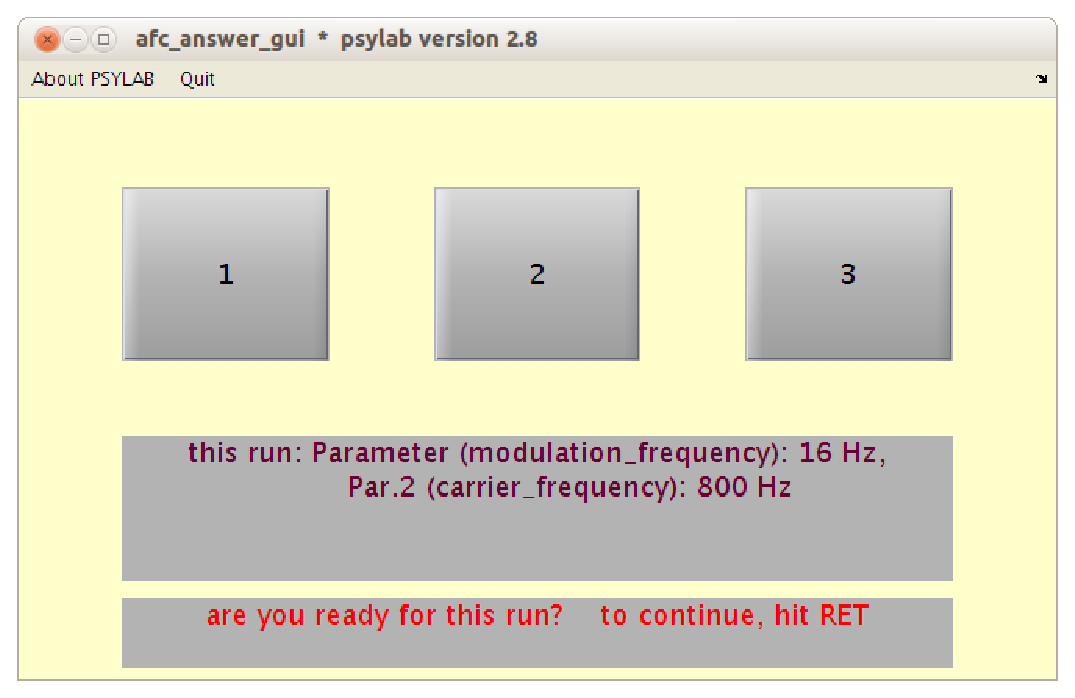
\includegraphics[width=0.65\textwidth]{example_3afcgui_psylab28a}
  \caption{Example of the graphical user interface for the subject.}
  \label{fig:example_3afc_gui}
\end{center}
\end{figure}%
%%

%% --------------------------------------------------
\subsection{Running your experiment}
\label{sec:run-your-experiment}

Once you have set up your three experiment files correctly, running
your experiment means running your main script.  You might want to
instruct your subjects to always identify themselves by the identical
user ID, for example, their initials, which must not contain any white-spaces.  All
data gathered from a subject will be saved in a cumulative fashion, on
a one-separate-file-per-subject basis, see section~\ref{sec:psydat-file}.

The subjects can run the experiment at their own pace.  They may answer in
one of the ways described in section~\ref{sec:test-subject-interface},
as specified by the experimenter.

Analysis of your data can be performed at any later time,
independently from the subject performing the measurement.



%% --------------------------------------------------
\subsection{Setting up interleaved-tracks experiments}
\label{sec:design-interleaved-tracks}

Designing an \index{run!with interleaved tracks}interleaved-tracks
experiment requires to write a main script, a set script, and a user
script as well.  Most things are just same as for a single-run
non-interleaved experiment, but the following exceptions apply:
\begin{enumerate}
\item The variable \code{M} needs to be an \emph{array}, instead of a
  scalar variable, the number of elements of \code{M} being equal to
  the desired number of simultaneous interleaved tracks of the
  experiment. 
  
  In the main script, it is \emph{not} necessary to copy all fields of
  the struct variable \texttt{M(1)} to those of \texttt{M(2)}, \texttt{M(3)},
  \ldots\ for the 2nd, 3rd, \ldots\ concurrent run.  Instead, it is
  sufficient to only assign the ``relevant'' fields of \texttt{M(2)},
  \texttt{M(3)}, \ldots\ , \texttt{M(end)}, i.e. those fields with a different content
  for a different run.  When doing this, any fields of
  \texttt{M(2:end)} that are left unspecified will be assigned with
  the same values as found in \texttt{M(1)} automatically.  (This is
  a specific feature of \psylab, not of Matlab.) 

\item The script \code{mpsy\_intrlv\_afc\_main.m} is called to control
  the whole interleaved AFC experiment, instead of \code{mpsy\_afc\_main.m}.

  Likewise, the script \code{mpsy\_intrlv\_match\_main.m} is called to
  control the whole interleaved matching experiment, instead of
  \code{mpsy\_match\_main.m}.
\end{enumerate}

%%
\begin{figure}[htbp]
\begin{center}
\begin{struktogramm}(120,80)[\texttt{mpsy\_intrlv\_afc\_main.m}]
  \assign{rename variable \texttt{M} into \texttt{MI}, ~  clear variable \texttt{M}}
  \while[8]{ \textbf{for} \code{i=1} to (number of interleaved tracks) }
     \assign{assign \code{M} $\leftarrow$ \code{MI(i)} }
     \sub{call \textit{set script} of current experiment}
    \assign{assign \code{MI(i)} $\leftarrow$ \code{M} }  \whileend
  \while[8]{ \textbf{while} (not all tracks completed) }
    \assign{select random track number $i$ among all incomplete tracks.}
    \assign{assign \code{M} $\leftarrow$ \code{MI (i)} }
    \sub{call \textit{user script} of current experiment}
    \assign{present signals \code{m\_ref} and \code{m\_test} in $n$-AFC manner}
    \assign{process subject response}
    \assign{apply adaptive rule, change \code{M.VAR} and \code{M.STEP} accordingly}
    \assign{check whether current track is completed}
    \assign{assign \code{MI(i)} $\leftarrow$ \code{M} }
  \whileend
  \assign{protocol all data, save results to \code{psydat}-file}
\end{struktogramm}
  \caption{Principle  flow diagram of an interleaved-tracks experiment, as controlled by the
    script \texttt{mpsy\_intrlv\_afc\_main.m}}
  \label{fig:principle-mpsy_intrlv_afc_main}
\end{center}
\end{figure}%
%%

The following example code illustrates how to set up an
interleaved-tracks experiment.  The example shows the main script for
the tone-in-broadband-noise experiment (see in the subdirectory
\texttt{examples)} in which a sinusoidal tone of different frequencies is
to be detected in a running broad band noise of fixed bandwidth and
level. 
%
\label{page:example-code-afc-interleaved}
\begin{verbatim}
mpsy_init;

M.EXPNAME      = mfilename;    % experiment name, very important to be set correctly!
M.NUM_PARAMS   = 2;            % number of parameters
M.PARAMNAME(1) = {'testtone_frequency'};
M.PARAMUNIT(1) = {'Hz'};
M.PARAMNAME(2) = {'noise_level'};
M.PARAMUNIT(2) = {'dB'};
M.VARNAME      = 'testtone_level';
M.VARUNIT      = 'dB';
M.TASK         = 'which interval contained the test signal (1,2,3)?  ';
M.MINSTEP      = 1 ;  % minumum step size, in units of M.VARUNIT
M.NAFC         = 3 ;  % number of forced choice intervals
M.ADAPT_METHOD = '1up_2down';   % select adaptive method: transformed 1-up-2-down
M.MAXREVERSAL  = 4 ;  % number of reversals required as stop criterion
M.FEEDBACK     = 1 ;  % 1/0  = yes/no
(...)
M.FS               = 48000; % sampling frequency
M.USE_GUI          = 1;     % use a GUI for user input

M.SNAME = input('\n\n please type your name (initials, no spaces, press RETURN at end) ','s');

tone_freqs = [ 200 400 800 1600 3200 6400 ]; 

% assign different parameter sets for interleaved tracks experiment
for kk = 1:length(tone_freqs),
    M(kk).PARAM(1) = tone_freqs(kk);
    M(kk).PARAM(2) = -30;            % use the same noise level for all freq.'s
end

mpsy_intrlv_afc_main;
\end{verbatim}

The first part looks exactly the same as for a single-run experiment.
The difference starts in the \code{for}-loop, where
\code{M(kk).PARAM(1)} and \code{M(kk).PARAM(2)} are assigned, thereby
rendering \code{M} into an array with \code{length(tone\_freqs)}
elements (in this case 6 elements).  After the \code{for}-loop, most
fields of \texttt{M(2:6)} are still empty (by standard Matlab
behaviour).  These fields will be filled in automatically by way of
the script \texttt{mpsy\_intrlv\_init.m} which is called inside
\texttt{mpsy\_intrlv\_afc\_main}. 


The script \texttt{mpsy\_intrlv\_afc\_main} will start an experiment
with a number of 6 interleaved tracks (in this example).  It needs to
be called only once and it will exit after the last of the concurrent
interleaved tracks has finished.
%
The principle organisation of an interleaved-tracks experiment is
illustrated by the flow diagram in Fig.~\ref{fig:principle-mpsy_intrlv_afc_main}.


Note that the set script and the user script of an experiment can
sometimes stay exactly the same as for a single-run experiment.
However, all variables (including signals) that need to be different
in the different tracks (i.e.\ different parameter settings) must
become a field variable of the current variable \code{M}.  Then, these
fields will be saved into the variable \code{MI}, as shown in the flow
diagram in Fig.~\ref{fig:principle-mpsy_intrlv_afc_main}.  For more
details, consult the source code of the files
\texttt{mpsy\_intrlv\_*.m} dealing with interleaved-tracks
experiments.
\\

The example of an interleaved-tracks experiment given on
page~\pageref{page:example-code-afc-interleaved} illustrated the use
of a number of concurrent parameter value(s) sets, i.e.\ different tone
frequencies in that case.  However, this is not the only possibility
offered by interleaved-tracks experiments in \psylab.  
Another example is given in the file(s)
\texttt{match\_freq\_binaural\_intrlv*.m} in the \code{examples} subdirectory. 

%% The following example code, taken from the example
%% \texttt{match\_freq\_binaural\_intrlv.m}, illustrates how you could
%% interleave tracks for different parameter sets \emph{and/or} with
%% different adaptive methods per track (with the aim to converge at
%% different values of percent correct responses).
%% %
%% \begin{verbatim}
%% ref_freqs = [1000 2000 400];
%% 
%% for freq = ref_freqs,
%%  
%%   M(1).PARAM(1) = freq;
%%   M(1).PARAM(2)  =  1;   % test signal side left
%%   M(1).ADAPT_METHOD = '1up_2down';
%%   % this resulting p_correct needs to be set manually to match content of ADAPT_METHOD. 
%%   M(1).PARAM(3) = 70.7;
%%  
%%   M(2).PARAM(1) = freq;
%%   M(2).PARAM(2)  =  1;   % test signal side left
%%   M(2).ADAPT_METHOD = '2up_1down';
%%   % this resulting p_correct needs to be set manually to match content of ADAPT_METHOD. 
%%   M(2).PARAM(3) = 29.3;
%% 
%%   mpsy_intrlv_match_main;
%% 
%% end
%% \end{verbatim}
%% This code will run three consecutive interleaved experiment, one for
%% each reference frequency.  Note in this example that you must specify
%% all values of the \code{PARAM} field of all elements of the vector
%% \code{M(:)} explicitly, while the other fields of \code{M(:)} that have
%% been left empty will be filled in automatically by way of the script
%% \code{mpsy\_intrlv\_init.m}.
%% \\
%% \emph{Note the use of the third parameter in this example}.  It is
%% necessary in this case because the definition of ``threshold'' (i.e.\
%% which percent correct is defined to correspond to ``threshold'') is not
%% otherwise documented in the psydat file.


When designing your own interleaved experiment with \psylab\ you will
probably need to study the files \code{mpsy\_intrlv\_*.m} in more
detail.  For example, specifying the following lines 
%
\begin{verbatim}
M(1).ADAPT_METHOD = '1up_2down';
M(2).ADAPT_METHOD = '2up_1down';
M(6).ADAPT_METHOD = '2up_1down';
\end{verbatim}
in the main script of some 6-interleaved-tracks experiment with
different adaptive rules in the different tracks would lead to an
auto-filled-in value of \verb+'1up_2down'+ for the field
\verb+ADAPT_METHOD+ of \code{M(3)} through \code{M(5)} as these fields
are empty so far.  This is carried out by \code{mpsy\_intrlv\_init.m}
which will always set empty fields to the corresponding value of
\code{M(1)}, being \verb+'1up_2down'+ in the above example.


%% --------------------------------------------------
\subsection{Avoid the use of built-in function {\tt sound} for playback}
\label{sec:avoid-builtin-sound}

Unfortunately, in Version 2011 of Matlab the audio handling was
redesigned in a way that made the built-in function \code{sound}
almost non-functioning.

While this bug was fixed again by Matlab, a somewhat nicer and
independent work-around for this annoying problem (and for others as
well) is to use an alternative method to send your audio samples to
your soundcard: ``\index{msound!alternative sound output}msound''.
\code{msound} is a mex-file, also developed at the IHA, that uses the
PortAudio-Interface (of \code{http://www.portaudio.com/}) for
communicating with your sound card.  More information about \code{msound} can
be found at the website of the Institute for Hearing Technology and
Audiology (http://www.hoertechnik-audiologie.de/, then look for
``Institut f�r H�rtechnik und Audiologie'' $\rightarrow$
``Software''), and on github.

The \code{msound} mex-file is now also included in the \psylab-distribution.
It comes in several pre-compiled versions for win, gnu/linux-systems
and mac, mostly in 32 and 64bit format.  The compiled binary files can also be
found on github under ``releases''.  The 'dll'-format (not on github any
longer) is needed for older Matlab versions on win32-system.  If you
encounter a warning about a ``shadowing'' effect of some msound-file
over another, e.g.\ the 'mexw32' version shadowing the 'dll' version, you
may just delete the 'dll' version.
%
In order to enable sound output via \code{msound}, only a few additional
\psylab-variables need to be set:
\begin{verbatim}
M.USE_MSOUND       = 1;     % flag whether or not to use msound (1 or 0)
M.MSOUND_DEVID     = 0;     % device ID for msound (choose 0 or [] for default device)
M.MSOUND_FRAMELEN  = 1024;  % framelen for msound (number of samples)
M.MSOUND_NCHAN     = 1;     % number of channels, must match  size(m_outsig,2)
\end{verbatim}

The variable \verb+M.USE_MSOUND+ works as a flag-variable whether or
not to use \code{msound} instead of \code{sound}.

The frame length \verb+M.MSOUND_FRAMELEN+ is the number of samples
within each frame of audio, also called block size, that is sent to
the soundcard.  You should test/experiment, which
\verb+M.MSOUND_FRAMELEN+ works best on your own system.  The value of
1024 worked well for most purposes on many machines/soundcards, but
maybe not for yours.

It is important to set the \verb+M.MSOUND_NCHAN+ to the number
of channels of your stimuli, i.e.\ 1 for mono/diotic and 2 for
stereo/dichotic signals.  If \verb+M.MSOUND_NCHAN+ does not match
\verb+size(m_outsig,2)+, an error will occur.

When using sound output via \code{msound} in \psylab, it is possible to
use the visual interval indication.  Put another way round, on some
systems it will only be   possible to use the visual interval indication \emph{if}
you use \code{msound} for sound output.  



%% --------------------------------------------------
\subsection{Debugging your experiment}
\label{sec:debug-your-experiment}

For purposes of \index{debugging!variable \texttt{M.DEBUG}}debugging,
set the variable \code{M.DEBUG} to a value larger than zero (1, 2, 3,
4), to get an increasing amount of temporary information and plots.
Stick to the rule: ``Use the force -- read the source'' to see the
behaviour in case of \code{M.DEBUG}$>$0.

When gathering real data with test subjects, however, you will want to
set \code{M.DEBUG=0;}




%% --------------------------------------------------
\section{Saving and analysing your experimental data}
\label{sec:saving-the-data}


%% --------------------------------------------------
\subsection{How your data are saved: the 'psydat' file}
\label{sec:psydat-file}

Each time when one run has been completed, i.e.\ a threshold has been
reached in an adaptive experiment or a block of trials in a constant
stimulus experiment has been finished, the result of that run is
automatically saved in a result file in ASCII-format.  The name of
that file is always formed by the common prefix '\texttt{psydat\_}'\,
followed by the value of \code{M.SNAME}, i.e.\ the subject name.  It
is important for correct functioning of \psylab\ to avoid any
whitespace characters in the subject name.
%
Example: \code{M.SNAME = 'mh'} yields the filename
\texttt{psydat\_mh}.  

The \index{psydat-file}psydat-file is written in a special fixed
format.  One important aspect of this format is the fact that all data
entries in the file are delimited by whitespace characters.
Consequently, this requires that certain \psylab-variables (for
example, parameter names or units) \emph{must not contain whitespace
  characters}.  You should not try to change this behaviour, as this
would likely interfere with the mechanism for analysis and display of
(all) results.  It is mandatory that the precise format of the psydat
file is maintained.  This means that comments, extra lines, or missing
lines are not allowed as these would very likely crash the mechanism
for automatic data extraction from the psydat file (see
section~\ref{sec:display-results}).


\subsubsection{Adaptive experiments}
\label{sec:psydat_adaptive-experiments}


The following data will be saved in the psydat-file after each
completion of one run: experiment name; subject name; date and time;
number of stimulus parameters; name, value, and unit of each
parameter; name of adaptive rule; name of stimulus variable, threshold value, its standard
deviation and minimal and maximal value, unit of stimulus variable.
The result entry of one run will span across 
several
%%\code{3+M.NUM\_PARAMS}
lines in the psydat-file.  Have a look into one of the example
psydat-files in the \texttt{examples} subdirectory.  One example entry
in the psydat file belonging to the experiment
\texttt{sam\_sincarrier\_detect.m} is the following:
%
\begin{verbatim}
##adapt## sam_sincarrier_detect mh 08-Jan-2006__18:46:03 npar 2 ####
%%----- PAR1: modulation_frequency 16.000000 Hz
%%----- PAR2: carrier_frequency 400.000000 Hz
%%----- ADAPT: 1up_2down 
  modulation_degree -31.000000 1.278275 -34.000000 -29.000000 dB
\end{verbatim}
%
This entry informs you that the subject named '\texttt{mh}' performed
the \emph{adapt}ive experiment '\texttt{sam\_sincarrier\_detect}' on the 8th of
January 2006 in the early evening.  The experiment had 2 parameters
which are specified in rows 2 and 3, and it used the adaptive
1-up-2-down rule.  The result was a threshold value 
at $m$=~-31\,dB, with a standard deviation of 1.28\,dB.  The minimal
respectively maximal values of the modulation degree during the
measurement phase were -34\,dB respectively -29\,dB.

The default behaviour of \psylab\ is to calculate the
\index{threshold!calculation of}\emph{threshold} of
an adaptive run as the \emph{median} of all values of \code{M.VAR} during the
measurement phase, and to output this value into the psydat file.
However, by setting the variable \code{M.SAVEMEAN} 
to 1 (meaning \emph{true}), you can change this and specify that the threshold should rather
be calculated as the \emph{mean} of all values of \code{M.VAR} during
the measurement phase.  The default behaviour can be achieved by
letting \code{M.SAVEMEAN} be an empty field or by setting it to the
value~0 (meaning \emph{false}).

The default behaviour of \psylab\ is to output only the resulting
threshold value of an adaptive run to the psydat-file.  However, by setting the variable
\code{M.SAVERUN} to 1, you can change this and specify that also all
values of \code{M.VAR} during the entire adaptive run, including the
corresponding answers of the subject, should be output to the
psydat-file in a separate line.   One entry in the file could then
look like this:
\begin{verbatim}
##adapt## sam_sincarrier_detect mh  22-Nov-2016__17:14:50 npar 2 ####
%%----- PAR1: modulation_frequency 16.000000 Hz
%%----- PAR2: carrier_frequency 800.000000 Hz
%%----- ADAPT: 1up_2down 
%%----- VAL: -8 1 -8 1 -12 1 -12 1 -16 1 -16 1 -20 1 -20 1 -24 1 -24 1 -28 0 -24 1 -24 1 -26 0 
-24 1 -24 1 -25 1 -25 1 -26 0 -25 1 -25 1 -26 0 -25 1 -25 1 -26 0 -25 1 -25 1
  modulation_degree -25.000000 0.492366 -26.000000 -25.000000 dB
\end{verbatim}
%
The line starting with \verb+%%----- VAL:+ informs you that the
subjects listened to stimuli with the following variable values
resp. modulations degrees (and gave answers in parentheses) during
this run:\\
-8~dB (correct); -8~dB (correct); -12~dB (correct); -12~dB (correct); -16~dB (correct); etc.
The run consisted of 27 trials, of which the last three were at
-26~dB (wrong); -25~dB (correct); -25~dB (correct).  



\subsubsection{Constant stimuli experiments}
\label{sec:psydat_conststim-experiments}

In case of a constant stimuli experiment, one experimental run will
produce several entries in the psydat-file, one per variable value.
An example entry, performed with the experiment
\texttt{jnd\_frequency.m}, looks like this:
%
\begin{verbatim}
##const## jnd_frequency mh 22-Mar-2017__12:55:13 npar 2 ####
%%----- PAR1: reference_frequency 250.000000 Hz
%%----- PAR2: tone_level -10.000000 dB
%%----- CONST: num_presentations 5 
  rel_frequency_increment 4.000000 cent   prob_correct 0.600000
##const## jnd_frequency mh 22-Mar-2017__12:55:13 npar 2 ####
%%----- PAR1: reference_frequency 250.000000 Hz
%%----- PAR2: tone_level -10.000000 dB
%%----- CONST: num_presentations 5 
  rel_frequency_increment 8.000000 cent   prob_correct 0.800000
##const## jnd_frequency mh 22-Mar-2017__12:55:13 npar 2 ####
%%----- PAR1: reference_frequency 250.000000 Hz
%%----- PAR2: tone_level -10.000000 dB
%%----- CONST: num_presentations 5 
  rel_frequency_increment 16.000000 cent   prob_correct 0.800000
##const## jnd_frequency mh 22-Mar-2017__12:55:13 npar 2 ####
%%----- PAR1: reference_frequency 250.000000 Hz
%%----- PAR2: tone_level -10.000000 dB
%%----- CONST: num_presentations 5 
  rel_frequency_increment 32.000000 cent   prob_correct 1.000000
\end{verbatim}
%
Note that these four entries were written to the psydat file at the
same time, namely after all 5 presentations for each of the four
different values of the variable (4, 8, 16, and 32 cent) were
completed.  These four data points can form a part of the psychometric
function.  Any calculation of thresholds or fitting of a psychometric
function from theses data is left to the user of \psylab.

For a constant stimulus experiment, the default behaviour of \psylab\
is to output the resulting pairs of variable/$P_{correct}$ to the
psydat-file.  As for an adaptive experiment, you can change this by
setting the variable \code{M.SAVERUN} to 1 to specify that also all
values of \code{M.VAR} during the entire constant stimuli run,
including the corresponding answers of the subject, should be output
to the psydat-file in a separate line.  One set of entries in the file could
then look like this:
%
\begin{verbatim}
##const## jnd_frequency mh 12-Mar-2019__15:40:42 npar 2 ####
%%----- PAR1: reference_frequency 250.000000 Hz
%%----- PAR2: tone_level -10.000000 dB
%%----- CONST: num_presentations 3 
  rel_frequency_increment 4.000000 cent   prob_correct 0.333333
##const## jnd_frequency mh 12-Mar-2019__15:40:42 npar 2 ####
%%----- PAR1: reference_frequency 250.000000 Hz
%%----- PAR2: tone_level -10.000000 dB
%%----- CONST: num_presentations 3 
  rel_frequency_increment 16.000000 cent   prob_correct 1.000000
##const## jnd_frequency mh 12-Mar-2019__15:40:42 npar 2 ####
%%----- PAR1: reference_frequency 250.000000 Hz
%%----- PAR2: tone_level -10.000000 dB
%%----- CONST: num_presentations 3 
%%----- VAL: 32 1 16 1 32 1 4 0 16 1 16 1 32 1 4 0 4 1
  rel_frequency_increment 32.000000 cent   prob_correct 1.000000
\end{verbatim}
%
In this short example, three different variable values (being 4, 16,
and 32 cent) were presented three times each.  Note that the line
starting with \verb+%%----- VAL:+ is present in the file only once,
close to the end of the last of the three entries.  However, it informs you about all
the 3$\cdot 3$=9 presented stimuli that produced the three entries,
one for 4 cent, 16 cent, and 32 cent as the stimulus variable.


~\\


Should you ever want to perform the same \psylab\ experiment both
using an adaptive method and also using the constant stimuli method,
then this is possible by just changing a few lines in the main script
of the experiment.  However, you should then use two different subject
names for the same subject, e.g. ``mh\textbf{a}'' for subject ``mh''
in the \textbf{a}daptive experiment and ``mh\textbf{c}'' in the
\textbf{c}onstant stimuli experiment.  This will allow the functions
described in section~\ref{sec:display-results} to keep the two
different kinds of results separate.



\subsubsection{psydat-file version}
\label{sec:psydat-file-version}


The data format of the psydat-file has seen several versions.  The
current psydat-file-version~``3'' has been in use since
\psylab-version~2.8.  The functions for reading the psydat-file
described in section~\ref{sec:display-results}
need to match with the format version of the psydat-file.
Section~\ref{sec:reading-old-psydat-files} explains how to read data
from an ``old'' psydat file that was produced with \psylab\ older than
version~2.8.   


\subsubsection{Temporary files}
\label{sec:temporary-files}

In addition to the psydat-file in ASCII format, the variables
\texttt{M} and \texttt{M\_*} can also get saved as a binary mat-file
each time a run has been completed.  This behaviour will only be turned on
if \code{M.DEBUG}$>$0.  However, this is mainly for rescue and special
purposes.  They will not be used by \psylab\ for later data analysis,
and so the binary files may as well be deleted.  If you do not need
these temporary files, just set \code{M.DEBUG=0;}.  When
\code{M.FEEDBACK}$>$1, then the functions
\code{mpsy\_plot\_feedback.m},  
\code{mpsy\_plot\_thresholds.m}, 
and 
\code{mpsy\_plot\_psycfunc.m}
will append a
copy of the resulting figure in eps format to a file named
\verb+'plot_*_+\textit{$<$subjectname$>$}' 



%% --------------------------------------------------
\subsection{Processing and displaying your results}
\label{sec:display-results}

Every time when a subject has completed one run, that run's result is
documented in the ``psydat'' file, see section~\ref{sec:psydat-file}.
All results can later be analysed and displayed in several ways by
using one of the following \psylab\ functions:

\begin{description}
\item[read\_psydat.m] Extract from the psydat file all those data
  points that belong to one subject and one experiment.
\item[display\_psydat\_raw.m] Plot all individual data points for one
  subject and one experiment. 
\item[display\_psydat.m] Plot all threshold results for one subject
  and one experiment, individually averaged across all repetitions for
  identical parameter value combinations.
\end{description}

These three functions are explained in the following subsections.


\subsubsection{read\_psydat.m}
\label{sec:read_psydat}


The script \index{psydat functions!read\_psydat.m}\code{read\_psydat.m} performs
the action to read the corresponding psydat file of the
subject and to extract from it all those lines that belong
to the given experiment name (and of course subject name).  Lines that
pertain to a different experiment are simply skipped by
\texttt{read\_psydat}.  The extracted data are returned in two different
data formats.  After the call 
\begin{verbatim}
[x,y] = read_psydat(s_name, exp_name) 
\end{verbatim}
variable \code{x} contains a struct variable with all data extracted
from the psydat file.  Each struct field is a vector or cell string
with as many elements as the number of data points in the psydat file.
A lot of information contained in \code{x} is therefore quite
redundant.  Variable \code{y} stores only the subset of numerical data
of \code{x}, in a matrix format which is explained in the verbose
output of \texttt{read\_psydat}.    See also the following section. 


\subsubsection{display\_psydat\_raw.m}
\label{sec:display_psydat_raw}

You can have a look at all individual data points that were
accumulated over time for one subject in an experiment.  In order to
plot \emph{all} data points \emph{individually}, use the script
\index{psydat functions!display\_psydat\_raw.m}\texttt{display\_psydat\_raw.m}. This
script makes use of \code{read\_psydat.m} internally.  Aside from
plotting, \texttt{display\_psydat\_raw.m} also returns the data that
were extracted from the psydat file in the same way as done by
\texttt{read\_psydat}.

The output from calling \texttt{display\_psydat\_raw.m} might look
like this and produce a plot as shown in
Fig.~\ref{fig:example_psydat_raw}:
%
\label{page:example_psydat_raw_data}
\begin{verbatim}
>> [x,y] = display_psydat_raw('mh', 'sam_sincarrier_detect')
*** info:  found 19 matching entries in psydat_mh
*** info:  meaning of the 6 cols of y:
           threshold, thres_sd, thres_min, thres_max, par1, par2 
x = 
         date: {1x19 cell}
          par: [1x2 struct]
      varname: {1x19 cell}
    threshold: [-31 -35 -48 -34 -29 -50 -31 -32 -32 -32 -34.5 -31 -40 -54 -32 -52 -32 -34 -31]
     thres_sd: [1x19 double]
    thres_min: [-34 -36 -50 -36 -30 -52 -33 -33 -36 -35 -35 -33 -42 -55 -33 -54 -34 -35 -32]
    thres_max: [-29 -32 -47 -32 -27 -49 -30 -28 -24 -29 -33 -30 -37 -53 -31 -51 -31 -33 -30]
      varunit: {1x19 cell}
y =
  1.0e+003 *
   -0.0310    0.0013   -0.0340   -0.0290    0.0160    0.4000
   -0.0350    0.0010   -0.0360   -0.0320    0.0640    0.4000
   -0.0480    0.0010   -0.0500   -0.0470    0.2560    0.4000
   -0.0340    0.0012   -0.0360   -0.0320    0.0160    1.6000
   -0.0290    0.0010   -0.0300   -0.0270    0.0640    1.6000
   -0.0500    0.0008   -0.0520   -0.0490    0.2560    1.6000
   -0.0310    0.0008   -0.0330   -0.0300    0.0160    3.2000
   -0.0320    0.0014   -0.0330   -0.0280    0.0640    3.2000
   -0.0320    0.0034   -0.0360   -0.0240    0.2560    3.2000
   -0.0320    0.0017   -0.0350   -0.0290    0.0160    0.4000
   -0.0345    0.0008   -0.0350   -0.0330    0.0160    1.6000
   -0.0310    0.0008   -0.0330   -0.0300    0.0160    0.4000
   -0.0400    0.0016   -0.0420   -0.0370    0.0640    0.4000
   -0.0540    0.0007   -0.0550   -0.0530    0.2560    0.4000
   -0.0320    0.0006   -0.0330   -0.0310    0.0640    1.6000
   -0.0520    0.0009   -0.0540   -0.0510    0.2560    1.6000
   -0.0320    0.0009   -0.0340   -0.0310    0.0160    3.2000
   -0.0340    0.0007   -0.0350   -0.0330    0.0640    3.2000
   -0.0310    0.0007   -0.0320   -0.0300    0.2560    3.2000
\end{verbatim}
As the experiment of this example comprised two parameters, the
output \code{y} has 4+2 columns. These are: threshold, standard deviation
of threshold, the minimal and maximal value of the stimulus variable
that occurred during the measurement phase, and the values of
parameter~1 and parameter~2.  Figure~\ref{fig:example_psydat_raw} shows
an errorbar-plot of the first and second column of \code{y} as a
function of the 5th column (parameter~1), separately for each value of
the 6th column (parameter~2), while columns 3 and 4 are not shown in
the plot. 


%%
\begin{figure}[htbp]
\begin{center}
  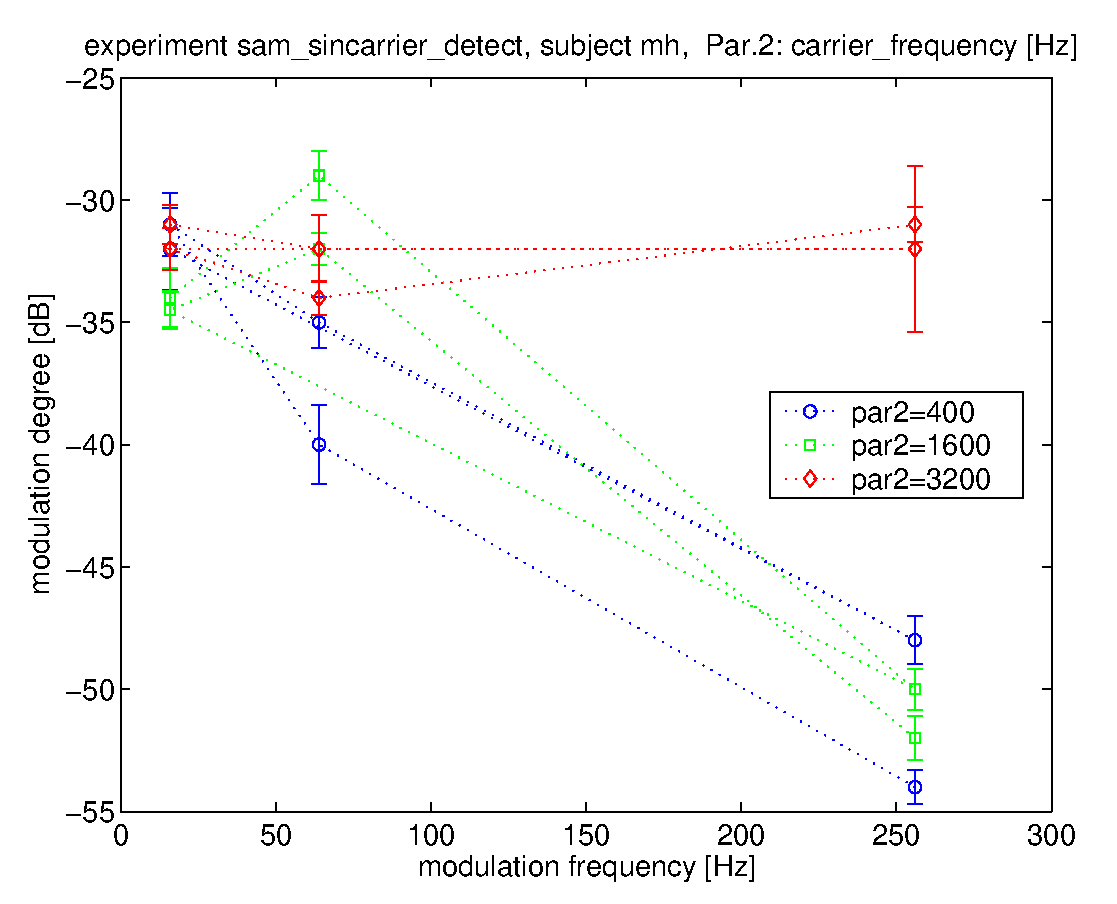
\includegraphics[width=0.7\textwidth]{example_psydat_raw}
   \caption{Example plot resulting from calling
     \texttt{display\_psydat\_raw}.  Every single data point
     (threshold) obtained by the subject is displayed separately. }
   \label{fig:example_psydat_raw}
\end{center}
\end{figure}%
%%

% %%
% \begin{figure}[htbp]
%  \begin{minipage}[t]{0.49\textwidth}
%   \centering
%    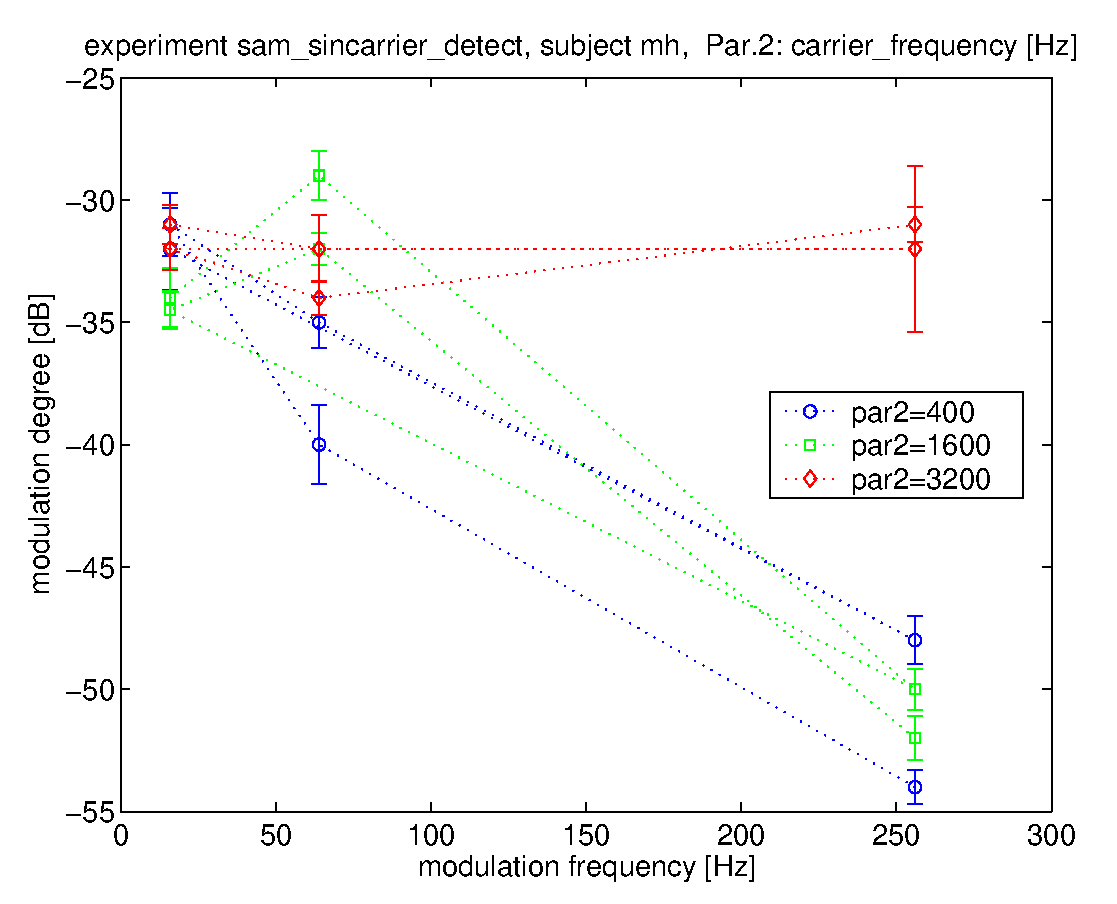
\includegraphics[width=1.0\textwidth]{example_psydat_raw}
%    \caption{Example plot resulting from calling
%      \texttt{display\_psydat\_raw}.  Every single data point
%      (threshold) obtained by the subject is displayed separately. }
%    \label{fig:example_psydat_raw}
%  \end{minipage}
%     \hspace{0.01\textwidth}
%  \begin{minipage}[t]{0.49\textwidth}
%   \centering
%    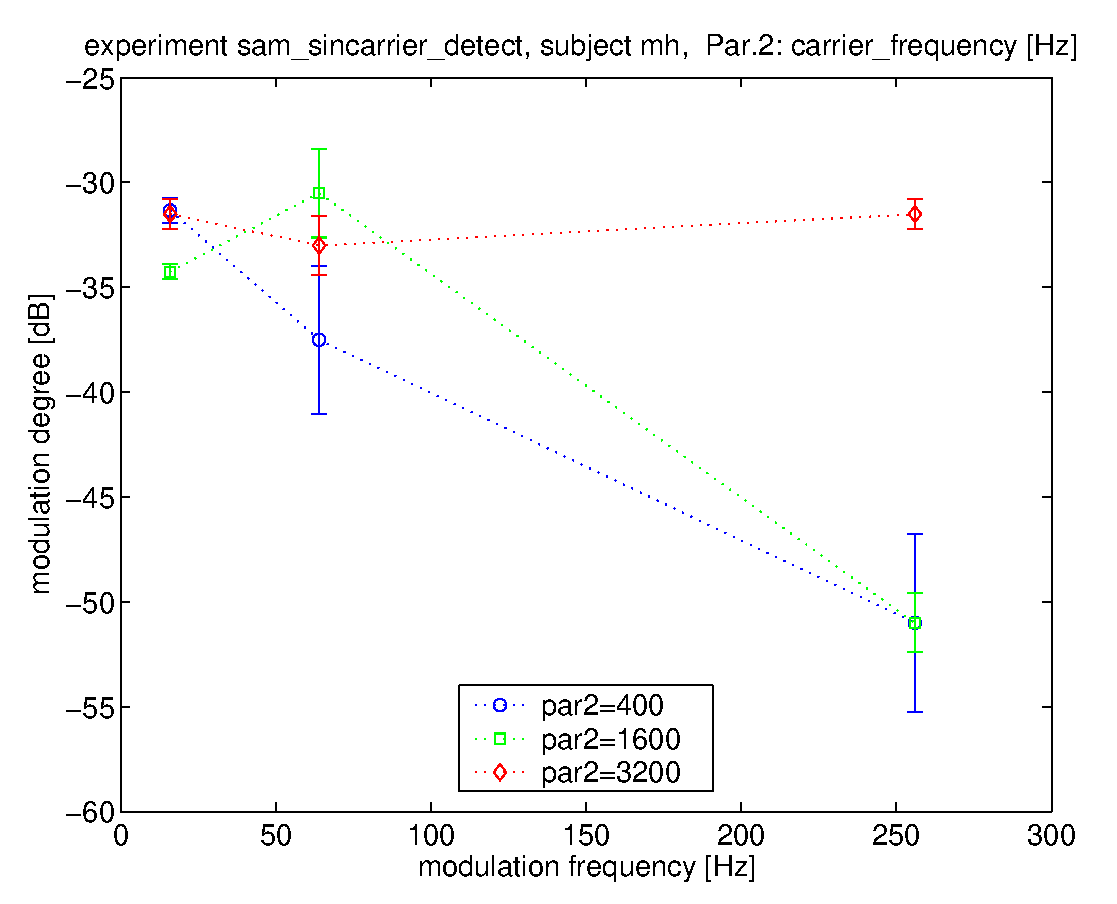
\includegraphics[width=1.0\textwidth]{example_psydat_average}
%    \caption{Example plot resulting from calling
%      \texttt{display\_psydat} for the same experiment and subject as
%      shown in Fig.~\ref{fig:example_psydat_raw}.  All data points
%      (thresholds) pertaining to repeated measurements with the same
%      set of parameter values have been averaged across prior to
%      plotting. }
%    \label{fig:example_psydat_average}
%  \end{minipage}
% \end{figure}%
% %%


\subsubsection{display\_psydat.m}
\label{sec:display_psydat}



The normal way to process and take a look at your experimental data
results is to use the function \index{psydat
  functions!display\_psydat.m}\code{display\_psydat.m}.  This function
makes use of \code{read\_psydat.m} to extract all corresponding data
from the psydat file.  Subsequently, the data handling differs for
adaptive experiments and constant stimuli experiments.
\\

%% --------------------------------------------------
\textbf{Adaptive experiments}

For an adaptive experiment, all thresholds that were measured
repeatedly are first averaged, individually per each (combination of)
different parameter value(s), and then plotted.  The first and second
argument of \code{display\_psydat} specify the subject name and
experiment name.

Calling \code{display\_psydat} with the same input arguments as for
\code{display\_psydat\_raw} produces four return arguments:
\begin{verbatim}
[x_all, y_average, y_ave2, hplot] = display_psydat(s_name, exp_name)
\end{verbatim}
The output \code{x\_all} contains the same data as described for
output \code{x} from \code{read\_psydat}, see above, but sorted by the
value of the 2nd parameter (and 3rd, 4th parameter, if present).
Output \code{y\_average} contains the same data as output \code{y} of
\code{read\_psydat}, but \emph{averaged} across repeated measurements
with the same set of parameter values.  Output \code{y\_ave2} contains
the same data as \code{y\_average}, but in a matrix format, where
each final data point to be plotted is contained in one row.  The
last output \code{hplot} contains an array of handles to all plot
lines in the figure.

%%
\begin{figure}[htbp]
\begin{center}
  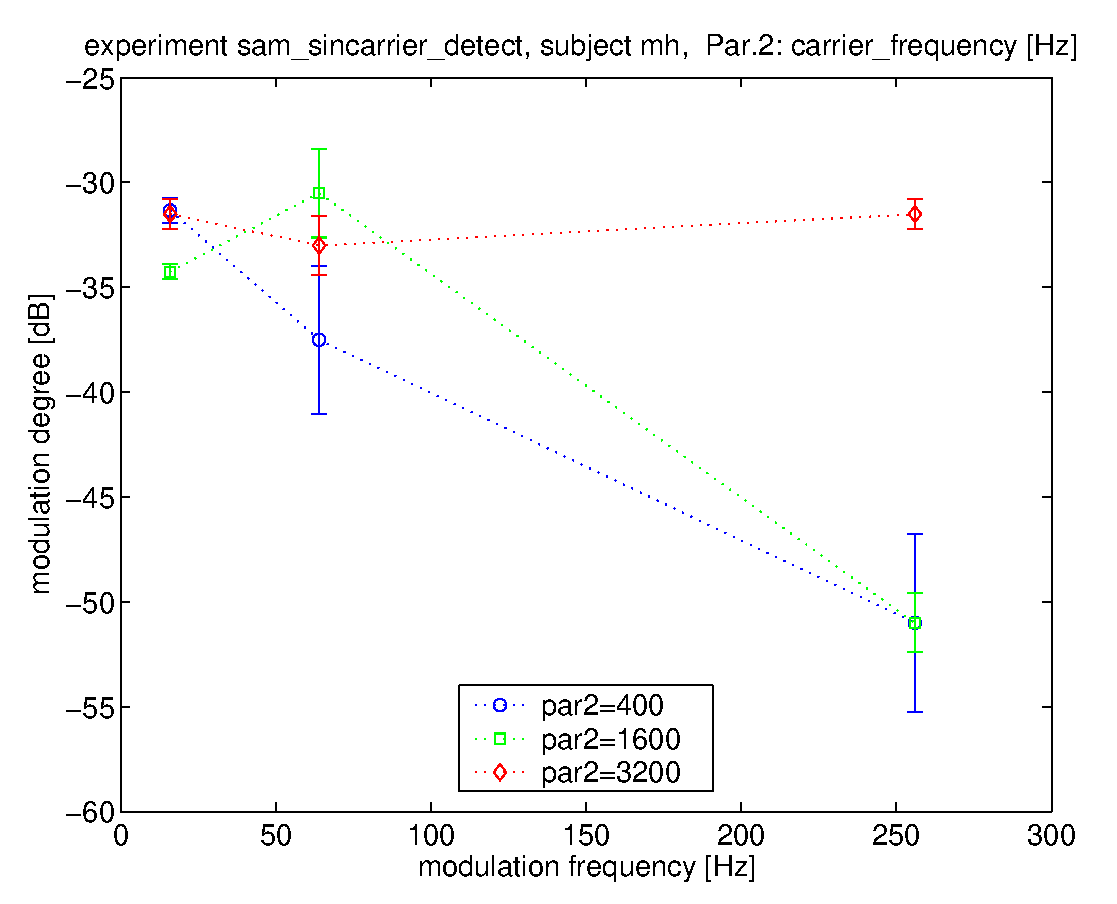
\includegraphics[width=0.7\textwidth]{example_psydat_average}
   \caption{Example plot resulting from calling
     \texttt{display\_psydat} for the same experiment and subject as
     shown in Fig.~\ref{fig:example_psydat_raw}.  All data points
     (thresholds) pertaining to repeated measurements with the same
     set of parameter values have been averaged across prior to
     plotting. }
   \label{fig:example_psydat_average}
\end{center}
\end{figure}%
%%

The output from calling \code{display\_psydat.m} might look like this
and produce a plot as shown in Fig.~\ref{fig:example_psydat_average}.
Compare this output and the data to those produced by
\code{display\_psydat\_raw.m} (see
page~\pageref{page:example_psydat_raw_data}).
\begin{verbatim}
>> [x_all,y_average,y_ave2] = display_psydat('mh', 'sam_sincarrier_detect')
*** info:  found 19 matching entries in psydat_mh
*** info:  meaning of the 6 cols of y:
           threshold, thres_sd, thres_min, thres_max, par1, par2 
x_all = 
1x3 struct array with fields:
    psydata
y_average = 
1x3 struct array with fields:
    psydata
y_ave2 =
  1.0e+003 *
   -0.0313    0.0006   -0.0340   -0.0293    0.0160    0.4000
   -0.0375    0.0035   -0.0390   -0.0345    0.0640    0.4000
   -0.0510    0.0042   -0.0525   -0.0500    0.2560    0.4000
   -0.0343    0.0004   -0.0355   -0.0325    0.0160    1.6000
   -0.0305    0.0021   -0.0315   -0.0290    0.0640    1.6000
   -0.0510    0.0014   -0.0530   -0.0500    0.2560    1.6000
   -0.0315    0.0007   -0.0335   -0.0305    0.0160    3.2000
   -0.0330    0.0014   -0.0340   -0.0305    0.0640    3.2000
   -0.0315    0.0007   -0.0340   -0.0270    0.2560    3.2000
\end{verbatim}
A comparison of \code{x\_all(1).psydata} and
\code{y\_average(1).psydata} respectively the first three rows of
\code{y\_ave2} illustrate the work of \code{display\_psydat}:
\begin{verbatim}
>> x_all(1).psydata
ans =
  -31.0000    1.2783  -34.0000  -29.0000   16.0000  400.0000
  -32.0000    1.6855  -35.0000  -29.0000   16.0000  400.0000
  -31.0000    0.7878  -33.0000  -30.0000   16.0000  400.0000
  -35.0000    1.0463  -36.0000  -32.0000   64.0000  400.0000
  -40.0000    1.6204  -42.0000  -37.0000   64.0000  400.0000
  -48.0000    0.9783  -50.0000  -47.0000  256.0000  400.0000
  -54.0000    0.7050  -55.0000  -53.0000  256.0000  400.0000
>> y_average(1).psydata
ans =
  -31.3333    0.5774  -34.0000  -29.3333   16.0000  400.0000
  -37.5000    3.5355  -39.0000  -34.5000   64.0000  400.0000
  -51.0000    4.2426  -52.5000  -50.0000  256.0000  400.0000
\end{verbatim}
Here, the values -31.3333 and 0.5774 in the first row of
\code{y\_average(1).psydata} (or of \code{y\_ave2}) are the mean
and the standard deviation across the thresholds that belong to the
three repetitions of the experiment with 1st parameter=16~Hz and 2nd
parameter=400~Hz.  The values -37.5000 and 3.5355 are the mean and
the standard deviation of the two repetitions belonging to 1st
parameter=64~Hz and 2nd parameter=400~Hz, etc.  

Note that the standard deviation of each experimental run, appearing
in the 2nd column of the output argument \code{x\_all(:).psydata}, is
\emph{neglected} by \code{display\_psydat} regarding the averaging
across repetitions.

Note also that the information about the adaptive rule belonging to
each data point is \emph{neglected} by \code{display\_psydat}
regarding the averaging across repetitions.  If you design an
experiment where you employ more than one adaptive rule, e.g.\
1-up-2-down and 2-up-1-down (with the aim to average the separate
thresholds belonging to the target probabilities of 70.7\% and 29.3\%)
then you need to store that piece of information in a different way.
It can be done by explicitly using a further parameter, as thresholds
belonging to different parameter values will be averaged separately by
\code{display\_psydat}.  As an example, the experiment
\code{match\_freq\_binaural\_singletrack} shows how this extra
parameter can be used.  
\\

%% --------------------------------------------------
\textbf{Constant stimuli experiments}

Also for a constant stimuli experiment, the first and second argument
of \code{display\_psydat} specify the subject name and experiment
name.  \code{display\_psydat} will first average across repeatedly
measured data (i.e.\ percentage correct values), individually per each
(combination of) different parameter value(s), and then plot them.
However, the averaging procedure and the output is different from that
for adaptive experiments.

One entry respectively one data set in the psydat-file contains the
``score'' $p$, i.e. the probability for a correct answer, and the
number $N$ of presentations from which this probability was obtained.

When a score $p$ was measured repeatedly, e.g.\ in repeated sessions
on different days, the individual scores are taken as indenpedent
measurements, and averaged using a weighting according the number of
presentations: Let the score $p_i$ be based on $N_i$ stimulus
presentations in measurement number $i$, with $i=1, \ldots, n$.  The
averaged score $\bar{p}$ is then calculated as $\bar{p} =\frac{\sum_i
  N_i\cdot p_i}{\sum_i N_i}$.  That means $\bar{p}$ is interpreted as
being based on a total number of $N_{tot} = \sum_i N_i$ stimulus
presentations.  A higher number of presentations will lead to a better
acuity of the estimate $\bar{p}$, e.g. as expressed by a smaller
standard error.  For a constant stimuli experiment,
\code{display\_psydat} will calculate both $\bar{p}$ and also the
standard error associated with $\bar{p}$, according to the following
reasoning:

Consider $N$ stimulus presentations where the stimulus variable was
held constant.  For each presentation, the subject's answer can either
be correct or wrong and it is assumed that the subjects's performance
is constant over time, which means that the probability $p$ for a
correct answer stays constant.  Let $X$ be the (random) number of
correct responses, then $X$ is distributed according to a Binomial or
``Bernoulli'' distrubtion with parameters $N$ and $p$: ~ $X\sim
Bi(N,p)$, with expectation value $E(X)=Np$ and variance
$Var(X)=Np(1-p)$.  Value $p$ is fixed but unknown, and shall therefore
be estimated.  The estimator of $p$ is then $\hat{p} = X/N$, which is
the relative occurrence of correct answers amoung all $N$
presentations.  It can be shown that $\hat{p}$ is an unbiased and
consistent estimator for $p$.  Also for repeated estimations of $p$,
the averaged score $\bar{p}$ is identical to the optimal estimator
$\hat{p}$ for the real (but unknown) value of $p$.  The random
variable $\hat{p}=\bar{p}$ can be interpreted as the \emph{average} of
a total number of $N_{tot}$ ones and zeros, with $X$ their sum.  The
expectation value of $\bar{p}$ is then $E(\hat{p})=E(\bar{p})=p$ and
the associated standard error, i.e.\ the standard deviation of
$\bar{p}$, is $\sigma_{\bar{p}}=\sqrt{\frac{1}{N^2} Var(X)} = \sqrt{p(1-p)/N}$.  These
two values are output by \code{display\_psydat}, separately for each
different combination of values of stimulus variable and stimulus
parameter(s).

The following example data from a constant stimuli experiment
with one parameter demonstrates this behaviour.  The psydat-file
contains the following data:
%
\begin{verbatim}
[x,y] = read_psydat('mm', 'demo_experiment')
*** info:  read_psydat found 37 matching entries in psydat_mm
*** info:  meaning of the 4 cols of y:
           prob_correct, num_presentations, variable, par1 
x = 
                 date: {1x37 cell}
                  par: [1x1 struct]
    num_presentations: [5 5 5 5 5 5 5 5 5 5 5 5 5 5 5 5 5 5 5 5 5 5 5 5 5 5 5 5 5 5 5 5 5 5 5 5 5]
              varname: {1x37 cell}
                  var: [1x37 double]
              varunit: {1x37 cell}
         prob_correct: [1x37 double]
y =
    0.8000    5.0000  -35.0000    0.0300
    0.8000    5.0000  -40.0000    0.0300
    1.0000    5.0000  -35.0000    0.0300
    0.8000    5.0000  -40.0000    0.0300
    0.6000    5.0000  -45.0000    0.0300
    0.8000    5.0000  -40.0000    0.0300
    0.8000    5.0000  -45.0000    0.0300
    0.8000    5.0000  -35.0000    0.0300
    0.6000    5.0000  -40.0000    0.0300
    0.4000    5.0000  -45.0000    0.0300
    1.0000    5.0000  -35.0000    0.0300
    0.4000    5.0000  -40.0000    0.0300
    0.8000    5.0000  -45.0000    0.0300
    0.8000    5.0000  -35.0000    0.0300
    0.6000    5.0000  -40.0000    0.0300
    0.6000    5.0000  -45.0000    0.0300
    1.0000    5.0000  -35.0000    0.0300
    0.6000    5.0000  -40.0000    0.0300
    0.8000    5.0000  -35.0000    0.0300
    1.0000    5.0000  -35.0000    0.0300
    1.0000    5.0000  -35.0000    0.0300
    1.0000    5.0000  -40.0000    0.0300
    0.4000    5.0000  -45.0000    0.0300
    1.0000    5.0000  -35.0000    0.0300
    0.8000    5.0000  -40.0000    0.0300
    0.6000    5.0000  -45.0000    0.0300
    1.0000    5.0000  -35.0000    0.0300
    1.0000    5.0000  -40.0000    0.0300
    0.2000    5.0000  -45.0000    0.0300
         0    5.0000  -50.0000    0.0300
    0.8000    5.0000  -38.0000    0.0300
         0    5.0000  -48.0000    0.0300
    1.0000    5.0000  -34.0000    0.0300
    0.8000    5.0000  -38.0000    0.0300
    0.8000    5.0000  -42.0000    0.0300
    0.4000    5.0000  -46.0000    0.0300
    0.4000    5.0000  -48.0000    0.0300
\end{verbatim}
%
The content of output variable $y$ shows that alls data point were
always measured with the same number of 5 stimulus presentations (2nd
column in \texttt{y}) and all measurements were made with the same
value of 0.03 for the first parameter M.PARAM(1) (4th column in
\texttt{y}).  The scores (which are proportions, resp. estimated
probabilities, all ranging between 0 and 1) are given in the 1st
column und the values of the stimulus variable (ranging between -50
and -34) are given in the 3rd column.

When these data are analzed by \code{display\_psydat\_raw}, the number $N$
of presentations and the score $p$ for each data point is taken to
calculate the standard error $\sigma_{\bar{p}}$ of the score $p$, as described above.  
The output then looks like this:
\begin{verbatim}
[x,y] = display_psydat_raw('mm', 'premasking_sinusoid_const')
*** info:  read_psydat found 37 matching entries in psydat_mm
*** info:  read_psydat: meaning of the 4 cols of 2nd output:
           prob_correct, num_presentations, variable, par1 
*** info:  display_psydat_raw: meaning of the 2nd column of 2nd output changed from
           number of presentations to estimated standard error of prob_correct
x = 
                    date: {1x37 cell}
                     par: [1x1 struct]
                 varname: {1x37 cell}
                     var: [1x37 double]
                 varunit: {1x37 cell}
            prob_correct: [1x37 double]
    std_err_prob_correct: [1x37 double]
y =
    0.8000    0.1789  -35.0000    0.0300
    0.8000    0.1789  -40.0000    0.0300
    1.0000         0  -35.0000    0.0300
    0.8000    0.1789  -40.0000    0.0300
    0.6000    0.2191  -45.0000    0.0300
...
\end{verbatim}
Only the first 5 lines of \texttt{y} are shown here.  As an example,
the value 0.1789 in the first line was calculated as
$\sqrt{0.8\cdot(1-0.8)/5}$, where 0.8 was the score and 5 was the number of presentations
(see first line of \texttt{y} in the output of \code{read\_psydat}).

For the same psydat-file, the output of \code{display\_psydat} then
looks like this:
\begin{verbatim}
[y_all, y_ave, y_ave2] = display_psydat('mm', 'premasking_sinusoid_const')
*** info:  read_psydat found 37 matching entries in psydat_mm
*** info:  read_psydat: meaning of the 4 cols of 2nd output:
           prob_correct, num_presentations, variable, par1 

*** info:  display_psydat: NOTE that for a constant stimulus experiment the output
           colums of read_psydat and display_psydat have different meanings, and 
           output y_all, y_average have different contents in their 2nd column:
           2nd col in y_all (1st output argument) contains  
          "num_presentations" of indiv. data, and 
           2nd col in y_average (2nd output argument) contains  
          "estimated std.err." of averaged data
y_all = 
    psydata: [37x4 double]
y_ave = 
    psydata: [9x4 double]
y_ave2 =
         0         0  -50.0000    0.0300
    0.2000    0.1265  -48.0000    0.0300
    0.4000    0.2191  -46.0000    0.0300
    0.5500    0.0787  -45.0000    0.0300
    0.8000    0.1789  -42.0000    0.0300
    0.7400    0.0620  -40.0000    0.0300
    0.8000    0.1265  -38.0000    0.0300
    0.9273    0.0350  -35.0000    0.0300
    1.0000         0  -34.0000    0.0300
\end{verbatim}


%% --------------------------------------------------
\subsubsection{Special effects: permute/change the look of your data with display\_psydat.m}
\label{sec:permuting-your-data}


\code{display\_psydat.m} offer an optional third and fourth argument.
They only take effect for experiments with more than one parameter:
the third argument specifies the ``plot style''.  A value of 1 means:
plot all data into one single figure.  A value of 2 means: use a new
figure for each value of the 2nd parameter (resp.\ for each unique
combination of values of the 2nd, 3rd, \ldots, $n$th parameter).
%%
\begin{figure}[htbp]
\begin{center}
  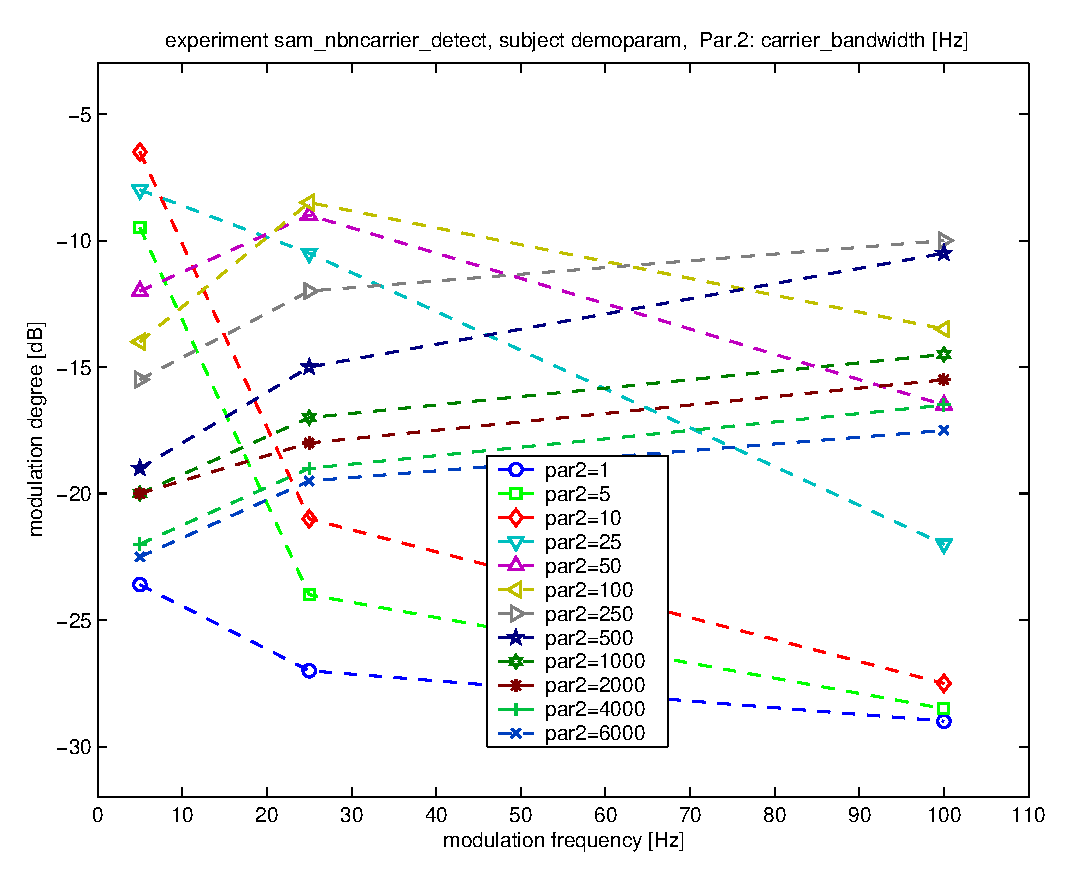
\includegraphics[width=0.7\textwidth]{demoparam_dau99}
  \caption{Example data of a modulation detection experiment as
    described in \cite{dau_1999a}
    % Dau \textit{et\,al.} 
    (see text).  These data have been taken from Fig.~1 in
    Dau\,\textit{et\,al.}
    %, JASA\,106(5), 2752--2760.  
    For clarity, standard deviations have been removed. }
  \label{fig:demoparam_dau99}
\end{center}
%\end{figure}% 
%%
%%
%\begin{figure}[htbp]
\begin{center}
  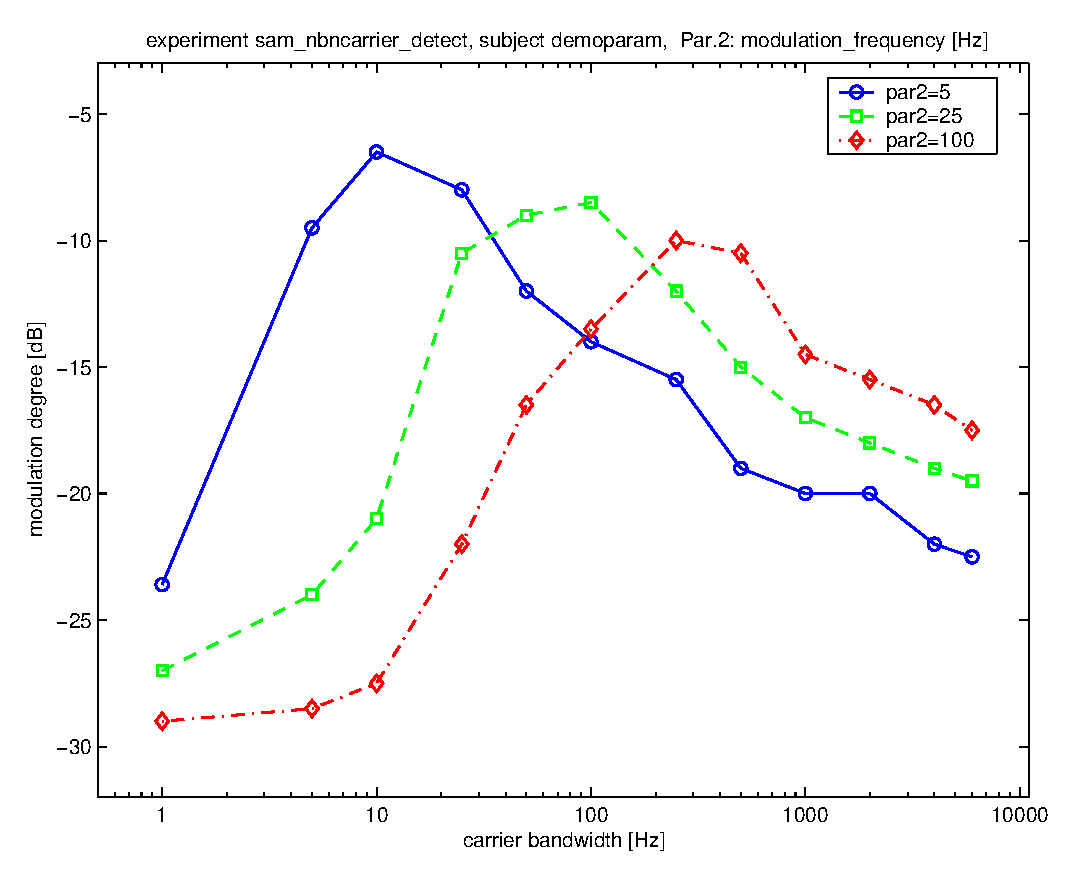
\includegraphics[width=0.7\textwidth]{demoparam_dau99_perm21}
  \caption{Replot of the same data as shown in
    Fig.~\ref{fig:demoparam_dau99} (See also Fig.~2 of
    Dau\,\textit{et\,al.} (1999)).  This plot was
  made by \code{display\_psydat} after permuting the order of the two
  parameters of the \psylab-experiment, see text.} 
  \label{fig:demoparam_dau99_perm21}
\end{center}
\end{figure}%
%%

The optional fourth argument of \code{display\_psydat} specifies a
permutation of parameters prior to further analysing and plotting
them.  The meaning of the fourth argument can best be explained by the
following examples.  Consider the modulation detection experiment of
Dau \textit{et\,al.}\cite{dau_1999a}.
%,(1999) (JASA\,106(5), 2752--2760).  
The Variables and Parameters could have been defined in the main
script as follows:

\begin{verbatim}
M.EXPNAME      = 'sam_nbncarrier_detect';    
M.NUM_PARAMS   = 2;
M.PARAMNAME(1) = {'modulation_frequency'};
M.PARAMUNIT(1) = {'Hz'};
M.PARAMNAME(2) = {'carrier_bandwidth'};
M.PARAMUNIT(2) = {'Hz'};
M.VARNAME      = 'modulation_degree';
M.VARUNIT      = 'dB';
\end{verbatim}

You might have measured the same thresholds as Dau \textit{et\,al.},
and calling \code{display\_psydat} like in  
%
%%[a,b,c,h] = display_psydat('demoparam', 'sam_nbncarrier_detect');
\begin{verbatim}
display_psydat('demoparam', 'sam_nbncarrier_detect');
\end{verbatim}
%
results in a plot as shown in Fig.~\ref{fig:demoparam_dau99}. 
%
Note here that threshold data (values of \code{M.VAR}) are plotted as
a function of the first parameter (values of \code{M.PARAM(1)}) in
Fig.~\ref{fig:demoparam_dau99}, and each value of the second
parameter (\code{M.PARAM(2)}) yields a separate curve.  This is the
standard behaviour of \code{display\_psydat}.  There are 12 curves for
the 12 individual values of the 2nd parameter (carrier bandwidth).

If you would like to replot your data so that threshold is plotted as
a function of carrier bandwidth, then you would need to permute the
numbering of your two parameters, prior to using
\code{display\_psydat}.  This can in fact be specified by the fourth
argument of this function, which must be a permutation of the numbers
1 through $n$, where $n$ is the number of parameters of your
experiment, i.e.\ \code{M.NUM\_PARAMS}. 
Calling \code{display\_psydat} like in  
%% [a,b,c,h] = display_psydat('demoparam', 'sam_nbncarrier_detect', 1, [2 1])
\begin{verbatim}
display_psydat('demoparam', 'sam_nbncarrier_detect', 1, [2 1])
set(gca, 'Xscale', 'log')
\end{verbatim}
%
% \begin{verbatim}
% [a,b,c,h] = display_psydat('demoparam', 'sam_nbncarrier_detect', 1, [2 1])
% delete(h(1,:));  % delete the errorbar lines 
% set(gca, 'Xscale', 'log')
% axis([0.5 11000 -32 -3])
% set(gca, 'XTick', [1 10 100 1000 10000])
% set(gca, 'XTickLabel', '1|10|100|1000|10000')
% \end{verbatim}
%
specifies that the original order of the parameters shall be permuted
into \verb+[2 1]+, i.e.\ the reverse order of the two parameters.  The
third argument, '1', specifies that all data should go into one single
plot figure.  The result is a plot like shown in
Fig.~\ref{fig:demoparam_dau99_perm21}.
%
Note here that only 3 curves are shown, namely one for each value of
the (originally first) parameter ``modulation frequency'', and each
curve is now made of 12 data points.  The modulation bandwidth now
acts as the first parameter in this plot and its title mentions the
modulation frequency as the second parameter.  
If the third argument (``plot style'') had been changed into 2 instead
of 1, then three separate figures would have resulted instead of the
single one shown in Fig.~\ref{fig:demoparam_dau99_perm21}.  


%% --------------------------------------------------
%\subsubsection{Too many psydat files, forgotten subject's names? use psydat\_helper.m}
\subsubsection{psydat\_helper.m}
\label{sec:psydat_helper}

After measuring a lot with \psylab, you will end up with a larger
number of psydat-files, or with very long psydat-files.  Eventually
you may loose an overview: Which data are stored where?  What was the
experiment called?  Which other experiments are stored in this
psydat-file?  When did the subject perform those measurements?

In this case you may get help from the tool
\code{psydat\_helper.m}. It opens a GUI and, after a click on the
``find all subject names''-button, display the subject names belonging
to \emph{all} psydat-files in the current directory.  Upon selecting
one of the subjects, a second list will pop up, showing \emph{all}
experiments that this subject has performed.  After selecting one of
them, clicking the ``plot all data''-button will extract and plot all
data belonging to this subject and experiment.  As an alternative, you
may select a subset of the data, ordered by the date of measurement as
shown in the rightmost list.  A click on the ``extract these and
plot''-button below will plot only the subset of data.  Data handling
and plotting is performed using the regular \code{display\_psydat.m},
as described earlier in this section.  A screenshot of the GUI is
shown in figure~\ref{fig:psydat_helper}.
%%
\begin{figure}[htbp]
\begin{center}
  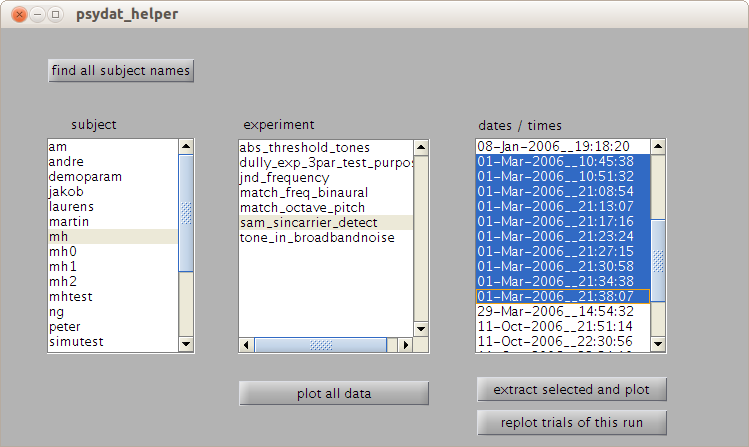
\includegraphics[width=0.8\textwidth]{psydat_helper_28a}
  \caption{Screenshot of the \code{psydat\_helper} GUI}
  \label{fig:psydat_helper}
\end{center}
\end{figure}%
%%


%% --------------------------------------------------
\subsubsection{Reading old psydat files}
\label{sec:reading-old-psydat-files}

Should you need to read a psydat file generated with an older version
of \psylab\, then the functions read\_psydat\_v2.m,
display\_psydat\_raw\_v2.m, and display\_psydat\_v2.m are available
for reading the data in the older psydat-file-version~2 (cf.\
section~\ref{sec:psydat-file-version}). 
 




%\clearpage
%% --------------------------------------------------
\section{Variables controlling \psylab}
\label{sec:variables-controlling-psylab}

\psylab\ is controlled by a number of \index{variables!reserved
  name}variables with a fixed, reserved name.  All of these variables
are struct fields of the variable with reserved name '\texttt{M}'.
Some of these variables are for internal purposes, while others need
to be specified by the user according to the needs of the current
experiment.

Table~\ref{tab:reserved-variables} contains a list of all
\psylab-variables, and explains their use.  It is important to
remember that some variables are required to be of a certain type, for example,
a string, a scalar or a cell string, or must not contain white-space
characters.  This is described in
section~\ref{sec:required-type-value-variables}.  The required type of
each variable is mentioned in parentheses after its name in
Table~\ref{tab:reserved-variables}. 

%\clearpage

\setlongtables
\begin{center}
\begin{longtable}{lp{0.7\textwidth}}
 \hline\multicolumn{2}{|c|}{user variables}\\
 \hline
\\
%% --------------------------------------------------
Name (type)              &  Meaning \\
% s=string, n=scalar number, \\
% v=vector, c=cell string\\
%% --------------------------------------------------
\hline
\hline
\code{M.SNAME}     (s)&
   subject name, as a string.  Preferably only initials.  \emph{Important}:  must
   not contain any white-space  characters.\\   
\code{M.EXPNAME}   (s)&
   experiment name.  The experiment name must be identical to the name
   of the main script (except for the extension '\texttt{.m}').  
\\
% --------------------------------------------------
\hline
\code{M.VAR}       (n)& 
   The value of the stimulus variable, as a scalar number, which is
   adaptively changed from trial to trial to find the subject's threshold. \\
\code{M.VARNAME} (s)&
   Name of the stimulus variable \texttt{M.VAR}, \eg 'test\_tone\_level'.\\ 
\code{M.VARUNIT} (s)&
   Unit of the stimulus variable \texttt{M.VAR}, \eg 'dB\_SPL'.\\ 
% --------------------------------------------------
\code{M.NUM\_PARAMS}    (n)&
   The number of stimulus parameters.  Must be equal to the length of
   \code{M.PARAM}. \\
\code{M.PARAM}     (v)& 
   The value resp.\ values, as a vector, of the stimulus parameter(s) which is/are kept
   constant during one run until threshold is reached.  In case of
   only one parameter, \code{M.PARAM} is of course a scalar. \\
\code{M.PARAMNAME} (c)&
   Name(s) of the  parameter(s), as cell strings, \eg 'frequency'. \\ 
\code{M.PARAMUNIT} (c)& 
   Unit(s) of the  parameter(s), \eg 'Hz'. \\
% --------------------------------------------------
\hline
\code{M.STEP} (n)& 
   Value of the current step size by which \code{M.VAR} will be
   changed adaptively depending on the subject's answer. \code{M.STEP}
   is specified in the same unit as \code{M.VAR}. \\ 
\code{M.MINSTEP} (n)& 
   Minimal value of the step size.  As soon as the condition
   \code{M.STEP} == \code{M.MINSTEP} has been reached, then
   \code{M.STEP} will not be reduced (halved) any longer and the
   measurement phase starts.  At that time, also the counter
   \code{M.REVERSAL} will be reset to  zero. \\ 
\code{M.MAXREVERSAL}   (n)& 
   Number of reversals == criterion for the termination of a run.  If
   the condition \code{M.MAXREVERSAL} == \code{M.REVERSALS} has been
   reached after the  measurement phase has begun, the run is terminated. \\
\code{M.NAFC}   (n) & 
   The number of $n$ of intervals in the $n$-AFC-task. \\
\code{M.ADAPT\_METHOD} (s)   \label{tab:item:m_adapt_method} &
   The name of the adaptive method of the up-down algorithm.  This
   name must be the suffix of one of the existing
   \code{mpsy\_adapt\_*.m} \psylab\ scripts, e.g. ``\code{1up\_2down}''
   for 1-up-2-down according to \cite{levitt_1971}, ``\code{wud}'' for the
   ``weighted up-down'' \cite{kaernbach_1991}, or
   ``\code{uwud}'' for the ``unforced weighted up-down'' \cite{kaernbach_2001}. \\
\code{M.PC\_CONVERGE} (n)   &
   The percentage correct towards which the adaptive methods ``wud''
   and ``uwud'' (see previous variable and
   subsection~\ref{sec:available-adapt-methods}) shall converge.
   Note, that a number between 0 and 1 is expected, not between 0 and
   100!  This variable is only used for the ``wud'' and ``uwud''
   methods.  \\ 
% \code{M.ADAPT\_N\_UP}  (n)&  
%    The number of successive wrong answers required for going
%    ``up'' in the adaptive transformed-up-down rule.\\
% \code{M.ADAPT\_N\_DOWN}   (n) & 
%    The number of successive correct answers required for going
%    ``down'' in the adaptive transformed-up-down rule.\\
%
\hline
% --------------------------------------------------
\code{M.CONSTSTIM\_ALLVARS} (v) & Vector containing all different (but
constant) values of \code{M.VAR} during the constant stimulus method. \\
\code{M.CONSTSTIM\_NUM\_} & Number of repeated presentations,
per each value in \\
~~~~\code{PRESENTATIONS} (n) & \code{M.CONSTSTIM\_ALLVARS}, during the constant stimulus method. \\
\hline
% --------------------------------------------------
\code{M.FS}        (n)& 
   The sampling frequency, in Hz. \\
\code{M.CALIB}     (v)& 
   Calibration constant = RMS level, in dB SPL, of a full-scale square
   wave.  Note that automatic calibration of your equipment is not yet part of \psylab. \\ 
\code{M.EARSIDE} (n) & 
   Variable specifying the presentation side in case the signals are
   generated purely mono.  Can take one of three predefined values: 
   \code{M\_BINAURAL} (default value, meaning \emph{diotic} presentation),
                       \code{M\_LEFTSIDE}, or  \code{M\_RIGHTSIDE}. \\  
\code{M.TASK}      (s)& 
   Task of the subject, as a string.  Typically something like ``Which
   interval contained the test signal?''\\
\code{M.FEEDBACK}  (n)& 
   Flag variable (1 or 0), whether or not to provide feedback to the
   subject  (\eg correct'/not correct') after each answer. \\
\code{M.USE\_GUI}  (n)& 
   Flag variable (1 or 0), whether or not to use a graphical user
   interface for the subject's answers instead of keyboard input.  \\
\code{M.VISUAL\_INDICATOR}     (n)& 
   Flag variable (1 or 0), whether or not to provide a visual
   indication of the individual $n$ intervals of each trial by
   colour-flashing the individual answer buttons.  Works
   only in case that \texttt{M.USE\_GUI} has been set, too.  \\
\code{M.INFO}     (n)&
   Flag variable to indicate whether or not additional information
   about the experiment should be provided to the subject.\\
\code{M.RESULTSTYLE}  (n)&
    Flag variable determining the style of resulting data plots
    directly after new data have been gathered.  A
    value of 1 (default) means: Plot all data into one figure.  Value
    2 means: use individual figures for each unique combination of
    parameter values. \\
\code{M.SAVEMEAN}  (n)&
    Flag variable to indicate that the threshold value should be
    calculated as the \emph{mean} across M.VAR for trials within the measurement
    phase, instead of the default behaviour, i.e., calculate their \emph{median} \\
\code{M.SAVERUN}  (n)&
    Flag variable to indicate that also all values of M.VAR and the
    corresponding answers of the subject should be output to the psydat-file\\
\code{M.DEBUG}     (n)& 
   Flag variable (0, or larger) to indicate the amount of intermediate
   information presented for debug purposes.  Should be set to 0 during real
   work measurements. \\
\hline
\code{M.USE\_MSOUND}  (n)& 
   Flag variable (0=default, or 1) to indicate that 'msound' should be used
   for sound output instead of Matlab's builtin 'sound'\\
\code{M.MSOUND\_DEVID}  (n)&
   The device ID of the sound card (i.e., a number) for use with msound.\\
\code{M.MSOUND\_FRAMELEN}  (n)&
   The number of samples of one frame/block for use with msound.  msound
   uses this length for internal buffering and the audio output is
   sent to the sound card in frames/blocks of this many samples.\\
\code{M.MSOUND\_NCHAN}  (n)&
   Number of channels for use with msound.  Mono signals have 1
   channel, stereo signals have 2, etc.  This value must match the value of
   \code{size(m\_outsig,2)}, otherwise an error will result.  
%% --------------------------------------------------
\\
\\
\\
\hline\multicolumn{2}{|c|}{internal variables - not to be manipulated
  by the user}\\
\hline
\\
%% --------------------------------------------------
Name (type)     &        Meaning \\
\hline
%% --------------------------------------------------
\code{M.QUIT}    (n)&  
   Flag variable indicting a complete termination of the current
   experiment. \\
\code{M.ACT\_ANSWER}   (n)&
   Current answer of the subject (1=correct, 0=wrong). \\
\code{M.LAST\_ANSWER}  (n)&
   Previous answer of the subject (1=correct, 0=wrong). \\
\code{M.REVERSAL}    (n)&
   Number of reversals in the current run.  Reversals are detected
   and counted automatically.  Counting starts at 0 again upon
   start of the measurement phase.\\
\code{M.REV\_IDX}    (v)&
   Indices (trial numbers of the current run) at which reversals
   are detected.  \\ 
\hline
\code{M.UA}    (n)&
   Current user answer in AFC experiments, i.e.\ the interval number,
   or special values requesting a quit of the run or the experiment.\\
\code{M.UD}    (n)&
   Current user answer in up-down experiment like in matching
   experiments.  Value~1 means 'down', value~2 means 'up'.\\
\code{M.ANSWERS}       (v)&
   Vector with all answers of the subject during the current run.\\
\code{M.STEPS} (v)&
   Vector with all values of \code{M.STEP}  during the current run.\\
% --------------------------------------------------
\code{M.VARS} (v)&
   Vector with all values of  \code{M.VAR}  during the current run.\\
% --------------------------------------------------
\code{M.ALLPARAM} (v)&
   Vector resp.\ matrix with all values of \code{M.PARAM} during the
   current experiment.  Each row of \code{M.ALLPARAM} contains the
   value(s) of \code{M.PARAM} pertaining to one run.\\
\code{M.ALLTHRES\_MED} (v)&
   Vector with all threshold values of the current experiment.  Each
   threshold is calculated from the values of \code{M.VARS} during
   each run.\\ 
\code{M.ALLTHRES\_STD} (v)&
   Vector with all value of the standard deviation of the thresholds
   during the current experiment.  Calculated from the values of
   \code{M.VARS} during each run.\\  
\code{M.DIRECTION}     (n)&
   Flag variable for the previous direction of change when applying
   adaptive up-down-rules.  Can take one of the predefined values \code{M.UP},
   \code{M\_DOWN}, or \code{M\_STAY}.\\
% \code{M.PSYDAT\_VERSION}   (n)&
%    Flag variable indicating the version number of the psydat file found in
%    the current directory. \\
% --------------------------------------------------
\hline\hline
\\
\caption{List of name and meaning of the \psylab-variables, to be
  specified by the user or for internal use.  The character in
  parentheses indicates the required variable type, i.e.\ s=string, n=scalar~number,
  v=vector, c=cell~string.}
  \label{tab:reserved-variables}
\end{longtable}
\end{center}






%% ============================================================
\section{Helpful scripts in \psylab}
\label{sec:helpful-scripts}

The \psylab\ distribution contains a few small additional functions
that are not needed directly by \psylab, but that can come in handy
for signal generation etc.  The following scripts/functions are also
described in their \texttt{help}.

\begin{description}

\item[ rms.m ]  Calculate RMS value of a signal vector.
  
\item[ gensin.m ] Generate sinusoidal tone.

\item[ hanwin.m ] Perform temporal windowing of a signal with a
  Hanning window resp.\ generate Hanning-window-shaped temporal ramps
  for onset- and offset of a signal. 
 
\item[ fft\_rect\_filt.m ] Function for very steep
  bandpass/notch filtering via FFT, by way of setting all Fourier
  components outside the passband to zero.

\end{description}



%% ============================================================
\section{New contributions to \psylab}
\label{sec:contributions}

Starting with version 2.1, a new directory \code{contrib} has been
added to the \psylab\ distribution.  It contains newly provided
contributions to \psylab.  These contributions comprise additional
features for \psylab, like new experimental paradigms, and
accompanying example experiments.

The contents of the \texttt{contrib} directory should be considered as
``experimental'' or beta-level-tested.  As time goes by and new
versions of \psylab\ are released, the new features might migrate to
become part of the regular \psylab-distribution.


The first two contributions were provided by students of ``Institut f�r
H�rtechnik und Audiologie''.  They implemented two new experimental
designs in \psylab, namely
\begin{enumerate}
\item A procedure to estimate several points on the psychometric
  function (that means: not only one threshold value) by repeatedly
  presenting stimuli at several fixed values of the stimulus variable,
  and recording the corresponding percent correct responses.  The
  accompanying example experiment is a replication of the binaural
  pitch detection and discrimination experiment by \cite{santurette_2007}
  %% Santurette \& Dau (Hear.~Res.~223, 2007)

  This has been replaced by new and extended code for the constant
  stimuli method.   

\item A closed-set 1-out-of-$n$ identification procedure.  The
  accompanying example experiment is a replication of the melody
  recognition experiment by \cite{akeroyd_2001}
  % Akeroyd et al. (JASA~110(3), 2001)
\end{enumerate}

Please note that the content of the contrib-directory is checked for
consistency with the remaining part of \psylab\ \emph{far less} frequently! 


\bibliography{mh-refs}
\bibliographystyle{apalike}

\printindex



%%% --------------------------------------------------
\addcontentsline{toc}{section}{GNU GPL}


\twocolumn
\tiny

\subsection*{The GNU GPL}
\label{sec:gnu-gpl}

~

\begin{verbatim}
		    GNU GENERAL PUBLIC LICENSE
		       Version 2, June 1991

 Copyright (C) 1989, 1991 Free Software Foundation, Inc.
     51 Franklin St, Fifth Floor, Boston, MA  02110-1301  USA
 Everyone is permitted to copy and distribute verbatim copies
 of this license document, but changing it is not allowed.

			    Preamble

  The licenses for most software are designed to take away your
freedom to share and change it.  By contrast, the GNU General Public
License is intended to guarantee your freedom to share and change free
software--to make sure the software is free for all its users.  This
General Public License applies to most of the Free Software
Foundation's software and to any other program whose authors commit to
using it.  (Some other Free Software Foundation software is covered by
the GNU Library General Public License instead.)  You can apply it to
your programs, too.

  When we speak of free software, we are referring to freedom, not
price.  Our General Public Licenses are designed to make sure that you
have the freedom to distribute copies of free software (and charge for
this service if you wish), that you receive source code or can get it
if you want it, that you can change the software or use pieces of it
in new free programs; and that you know you can do these things.

  To protect your rights, we need to make restrictions that forbid
anyone to deny you these rights or to ask you to surrender the rights.
These restrictions translate to certain responsibilities for you if you
distribute copies of the software, or if you modify it.

  For example, if you distribute copies of such a program, whether
gratis or for a fee, you must give the recipients all the rights that
you have.  You must make sure that they, too, receive or can get the
source code.  And you must show them these terms so they know their
rights.

  We protect your rights with two steps: (1) copyright the software, and
(2) offer you this license which gives you legal permission to copy,
distribute and/or modify the software.

  Also, for each author's protection and ours, we want to make certain
that everyone understands that there is no warranty for this free
software.  If the software is modified by someone else and passed on, we
want its recipients to know that what they have is not the original, so
that any problems introduced by others will not reflect on the original
authors' reputations.

  Finally, any free program is threatened constantly by software
patents.  We wish to avoid the danger that redistributors of a free
program will individually obtain patent licenses, in effect making the
program proprietary.  To prevent this, we have made it clear that any
patent must be licensed for everyone's free use or not licensed at all.

  The precise terms and conditions for copying, distribution and
modification follow.

		    GNU GENERAL PUBLIC LICENSE
   TERMS AND CONDITIONS FOR COPYING, DISTRIBUTION AND MODIFICATION

  0. This License applies to any program or other work which contains
a notice placed by the copyright holder saying it may be distributed
under the terms of this General Public License.  The "Program", below,
refers to any such program or work, and a "work based on the Program"
means either the Program or any derivative work under copyright law:
that is to say, a work containing the Program or a portion of it,
either verbatim or with modifications and/or translated into another
language.  (Hereinafter, translation is included without limitation in
the term "modification".)  Each licensee is addressed as "you".

Activities other than copying, distribution and modification are not
covered by this License; they are outside its scope.  The act of
running the Program is not restricted, and the output from the Program
is covered only if its contents constitute a work based on the
Program (independent of having been made by running the Program).
Whether that is true depends on what the Program does.

  1. You may copy and distribute verbatim copies of the Program's
source code as you receive it, in any medium, provided that you
conspicuously and appropriately publish on each copy an appropriate
copyright notice and disclaimer of warranty; keep intact all the
notices that refer to this License and to the absence of any warranty;
and give any other recipients of the Program a copy of this License
along with the Program.

You may charge a fee for the physical act of transferring a copy, and
you may at your option offer warranty protection in exchange for a fee.

  2. You may modify your copy or copies of the Program or any portion
of it, thus forming a work based on the Program, and copy and
distribute such modifications or work under the terms of Section 1
above, provided that you also meet all of these conditions:

    a) You must cause the modified files to carry prominent notices
    stating that you changed the files and the date of any change.

    b) You must cause any work that you distribute or publish, that in
    whole or in part contains or is derived from the Program or any
    part thereof, to be licensed as a whole at no charge to all third
    parties under the terms of this License.

    c) If the modified program normally reads commands interactively
    when run, you must cause it, when started running for such
    interactive use in the most ordinary way, to print or display an
    announcement including an appropriate copyright notice and a
    notice that there is no warranty (or else, saying that you provide
    a warranty) and that users may redistribute the program under
    these conditions, and telling the user how to view a copy of this
    License.  (Exception: if the Program itself is interactive but
    does not normally print such an announcement, your work based on
    the Program is not required to print an announcement.)

These requirements apply to the modified work as a whole.  If
identifiable sections of that work are not derived from the Program,
and can be reasonably considered independent and separate works in
themselves, then this License, and its terms, do not apply to those
sections when you distribute them as separate works.  But when you
distribute the same sections as part of a whole which is a work based
on the Program, the distribution of the whole must be on the terms of
this License, whose permissions for other licensees extend to the
entire whole, and thus to each and every part regardless of who wrote it.

Thus, it is not the intent of this section to claim rights or contest
your rights to work written entirely by you; rather, the intent is to
exercise the right to control the distribution of derivative or
collective works based on the Program.

In addition, mere aggregation of another work not based on the Program
with the Program (or with a work based on the Program) on a volume of
a storage or distribution medium does not bring the other work under
the scope of this License.

  3. You may copy and distribute the Program (or a work based on it,
under Section 2) in object code or executable form under the terms of
Sections 1 and 2 above provided that you also do one of the following:

    a) Accompany it with the complete corresponding machine-readable
    source code, which must be distributed under the terms of Sections
    1 and 2 above on a medium customarily used for software interchange; or,

    b) Accompany it with a written offer, valid for at least three
    years, to give any third party, for a charge no more than your
    cost of physically performing source distribution, a complete
    machine-readable copy of the corresponding source code, to be
    distributed under the terms of Sections 1 and 2 above on a medium
    customarily used for software interchange; or,

    c) Accompany it with the information you received as to the offer
    to distribute corresponding source code.  (This alternative is
    allowed only for noncommercial distribution and only if you
    received the program in object code or executable form with such
    an offer, in accord with Subsection b above.)

The source code for a work means the preferred form of the work for
making modifications to it.  For an executable work, complete source
code means all the source code for all modules it contains, plus any
associated interface definition files, plus the scripts used to
control compilation and installation of the executable.  However, as a
special exception, the source code distributed need not include
anything that is normally distributed (in either source or binary
form) with the major components (compiler, kernel, and so on) of the
operating system on which the executable runs, unless that component
itself accompanies the executable.

If distribution of executable or object code is made by offering
access to copy from a designated place, then offering equivalent
access to copy the source code from the same place counts as
distribution of the source code, even though third parties are not
compelled to copy the source along with the object code.

  4. You may not copy, modify, sublicense, or distribute the Program
except as expressly provided under this License.  Any attempt
otherwise to copy, modify, sublicense or distribute the Program is
void, and will automatically terminate your rights under this License.
However, parties who have received copies, or rights, from you under
this License will not have their licenses terminated so long as such
parties remain in full compliance.

  5. You are not required to accept this License, since you have not
signed it.  However, nothing else grants you permission to modify or
distribute the Program or its derivative works.  These actions are
prohibited by law if you do not accept this License.  Therefore, by
modifying or distributing the Program (or any work based on the
Program), you indicate your acceptance of this License to do so, and
all its terms and conditions for copying, distributing or modifying
the Program or works based on it.

  6. Each time you redistribute the Program (or any work based on the
Program), the recipient automatically receives a license from the
original licensor to copy, distribute or modify the Program subject to
these terms and conditions.  You may not impose any further
restrictions on the recipients' exercise of the rights granted herein.
You are not responsible for enforcing compliance by third parties to
this License.

  7. If, as a consequence of a court judgment or allegation of patent
infringement or for any other reason (not limited to patent issues),
conditions are imposed on you (whether by court order, agreement or
otherwise) that contradict the conditions of this License, they do not
excuse you from the conditions of this License.  If you cannot
distribute so as to satisfy simultaneously your obligations under this
License and any other pertinent obligations, then as a consequence you
may not distribute the Program at all.  For example, if a patent
license would not permit royalty-free redistribution of the Program by
all those who receive copies directly or indirectly through you, then
the only way you could satisfy both it and this License would be to
refrain entirely from distribution of the Program.

If any portion of this section is held invalid or unenforceable under
any particular circumstance, the balance of the section is intended to
apply and the section as a whole is intended to apply in other
circumstances.

It is not the purpose of this section to induce you to infringe any
patents or other property right claims or to contest validity of any
such claims; this section has the sole purpose of protecting the
integrity of the free software distribution system, which is
implemented by public license practices.  Many people have made
generous contributions to the wide range of software distributed
through that system in reliance on consistent application of that
system; it is up to the author/donor to decide if he or she is willing
to distribute software through any other system and a licensee cannot
impose that choice.

This section is intended to make thoroughly clear what is believed to
be a consequence of the rest of this License.

  8. If the distribution and/or use of the Program is restricted in
certain countries either by patents or by copyrighted interfaces, the
original copyright holder who places the Program under this License
may add an explicit geographical distribution limitation excluding
those countries, so that distribution is permitted only in or among
countries not thus excluded.  In such case, this License incorporates
the limitation as if written in the body of this License.

  9. The Free Software Foundation may publish revised and/or new versions
of the General Public License from time to time.  Such new versions will
be similar in spirit to the present version, but may differ in detail to
address new problems or concerns.

Each version is given a distinguishing version number.  If the Program
specifies a version number of this License which applies to it and "any
later version", you have the option of following the terms and conditions
either of that version or of any later version published by the Free
Software Foundation.  If the Program does not specify a version number of
this License, you may choose any version ever published by the Free Software
Foundation.

  10. If you wish to incorporate parts of the Program into other free
programs whose distribution conditions are different, write to the author
to ask for permission.  For software which is copyrighted by the Free
Software Foundation, write to the Free Software Foundation; we sometimes
make exceptions for this.  Our decision will be guided by the two goals
of preserving the free status of all derivatives of our free software and
of promoting the sharing and reuse of software generally.

			    NO WARRANTY

  11. BECAUSE THE PROGRAM IS LICENSED FREE OF CHARGE, THERE IS NO WARRANTY
FOR THE PROGRAM, TO THE EXTENT PERMITTED BY APPLICABLE LAW.  EXCEPT WHEN
OTHERWISE STATED IN WRITING THE COPYRIGHT HOLDERS AND/OR OTHER PARTIES
PROVIDE THE PROGRAM "AS IS" WITHOUT WARRANTY OF ANY KIND, EITHER EXPRESSED
OR IMPLIED, INCLUDING, BUT NOT LIMITED TO, THE IMPLIED WARRANTIES OF
MERCHANTABILITY AND FITNESS FOR A PARTICULAR PURPOSE.  THE ENTIRE RISK AS
TO THE QUALITY AND PERFORMANCE OF THE PROGRAM IS WITH YOU.  SHOULD THE
PROGRAM PROVE DEFECTIVE, YOU ASSUME THE COST OF ALL NECESSARY SERVICING,
REPAIR OR CORRECTION.

  12. IN NO EVENT UNLESS REQUIRED BY APPLICABLE LAW OR AGREED TO IN WRITING
WILL ANY COPYRIGHT HOLDER, OR ANY OTHER PARTY WHO MAY MODIFY AND/OR
REDISTRIBUTE THE PROGRAM AS PERMITTED ABOVE, BE LIABLE TO YOU FOR DAMAGES,
INCLUDING ANY GENERAL, SPECIAL, INCIDENTAL OR CONSEQUENTIAL DAMAGES ARISING
OUT OF THE USE OR INABILITY TO USE THE PROGRAM (INCLUDING BUT NOT LIMITED
TO LOSS OF DATA OR DATA BEING RENDERED INACCURATE OR LOSSES SUSTAINED BY
YOU OR THIRD PARTIES OR A FAILURE OF THE PROGRAM TO OPERATE WITH ANY OTHER
PROGRAMS), EVEN IF SUCH HOLDER OR OTHER PARTY HAS BEEN ADVISED OF THE
POSSIBILITY OF SUCH DAMAGES.

		     END OF TERMS AND CONDITIONS

	    How to Apply These Terms to Your New Programs

  If you develop a new program, and you want it to be of the greatest
possible use to the public, the best way to achieve this is to make it
free software which everyone can redistribute and change under these terms.

  To do so, attach the following notices to the program.  It is safest
to attach them to the start of each source file to most effectively
convey the exclusion of warranty; and each file should have at least
the "copyright" line and a pointer to where the full notice is found.

    <one line to give the program's name and a brief idea of what it does.>
    Copyright (C) <year>  <name of author>

    This program is free software; you can redistribute it and/or modify
    it under the terms of the GNU General Public License as published by
    the Free Software Foundation; either version 2 of the License, or
    (at your option) any later version.

    This program is distributed in the hope that it will be useful,
    but WITHOUT ANY WARRANTY; without even the implied warranty of
    MERCHANTABILITY or FITNESS FOR A PARTICULAR PURPOSE.  See the
    GNU General Public License for more details.

    You should have received a copy of the GNU General Public License
    along with this program; if not, write to the Free Software
    Foundation, Inc., 51 Franklin St, Fifth Floor, Boston, MA  02110-1301  USA


Also add information on how to contact you by electronic and paper mail.

If the program is interactive, make it output a short notice like this
when it starts in an interactive mode:

    Gnomovision version 69, Copyright (C) year name of author
    Gnomovision comes with ABSOLUTELY NO WARRANTY; for details type `show w'.
    This is free software, and you are welcome to redistribute it
    under certain conditions; type `show c' for details.

The hypothetical commands `show w' and `show c' should show the appropriate
parts of the General Public License.  Of course, the commands you use may
be called something other than `show w' and `show c'; they could even be
mouse-clicks or menu items--whatever suits your program.

You should also get your employer (if you work as a programmer) or your
school, if any, to sign a "copyright disclaimer" for the program, if
necessary.  Here is a sample; alter the names:

  Yoyodyne, Inc., hereby disclaims all copyright interest in the program
  `Gnomovision' (which makes passes at compilers) written by James Hacker.

  <signature of Ty Coon>, 1 April 1989
  Ty Coon, President of Vice

This General Public License does not permit incorporating your program into
proprietary programs.  If your program is a subroutine library, you may
consider it more useful to permit linking proprietary applications with the
library.  If this is what you want to do, use the GNU Library General
Public License instead of this License.
\end{verbatim}


\end{document}
% End of psylab-doc.tex

% Local Variables:
% time-stamp-pattern: "40/Updated:  <%2d %3b %:y %02H:%02M, %u>"
% TeX-master: t
% End:


 
